\documentclass[11pt, a4paper]{article}
\usepackage{graphicx} % Required for inserting images
\usepackage{caption} % for captions
\usepackage{bbm} % Math font; use \mathbbm{}
\usepackage[acronym]{glossaries} % for acronyms
\usepackage{physics} % Physics symbols

% \usepackage{showlabels} % To show equations labels on the PDF. Comment at the end

% Defining acronyms
\newacronym{etk}{ETK}{Einstein Toolkit}
\newacronym{tov}{TOV}{Tolman-Oppenheimer-Volkoff}
\newacronym{ns}{NS}{neutron star}
\newacronym{iu}{IU}{internal units}
\newacronym{eos}{EOS}{equation of state}
\newacronym{mol}{MoL}{Method of Lines}
\newacronym{pde}{PDE}{partial differential equation}
\newacronym{pdes}{PDEs}{partial differential equations}
\newacronym{ode}{ODE}{ordinary differential equation}
\newacronym{odes}{ODEs}{ordinary differential equations}
\newacronym{rk}{RK}{Runge-Kutta}
\newacronym{tvd}{TVD}{total variation diminishing}
\newacronym{ppm}{PPM}{piecewise parabolic method}

% Defining variables
\newcommand\figifcap{Initial and final conditions}
\newcommand\figrescompcap{Resolution comparison}

\title{Numerical Relativity Homework 2}
\author{Federico Leto di Priolo}
\date{June 2024}

\begin{document}

\maketitle

\section{Sod Shock Tube Problem} \label{sec:sod_main}

The Sod shock tube problem consists of a one-dimensional Riemann problem with initial discontinuities in density and pressure. The time evolution of the system can be computed by solving the Euler equations. Since the solution to this problem can be computed exactly, it is useful
for testing the accuracy of numerical codes. In this exercise, we solve the Sod problem with the \acrfull{etk} using different resolutions and compare the results with the exact solution.

The solution to the problem is described by three characteristics, each related to the propagation speed of the fluid in different regions. These can be associated with either a rarefaction wave, a shock wave, or a contact discontinuity. Specifically, the pressure and the velocity of the fluid develop a rarefaction wave and a shock wave, while the density also develops a contact discontinuity. The exact solution along with the initial conditions is shown in Figure \ref{fig:all_exact_if}.

For the numerical solutions, the HLLE Riemann solver has been used, along with the Minmod slope limiter. The domain extends in the range
\([-0.5, 0.5]\), and the evolution proceeds up to time \(t = 0.4\). The grid spacings used are \(\{0.005, 0.0025, 0.00125, 0.000625\}\), corresponding respectively to \(\{200, 400, 800, 1600\}\) grid points.

\subsection{Highest Resolution: 1600 points} \label{sec:highres1600}

We will use the results obtained with the highest resolution to showcase how the numerical solutions look. Figure \ref{fig:all_1600_snapshots} shows some snapshots of the profiles of density, pressure, and velocity of the fluid, including the initial and the final ones. As can be seen, S and CD waves travel in opposite directions with respect to the R waves. We point out that the fact that the initial profile in Figure \ref{fig:all_1600_snapshots} doesn't perfectly resemble a step (as it should) is due to the way the numerical results are interpolated on the chosen uniform grid \([-0.45, 0.45]\). Interpolation effects are also present in the final profile, though they are less evident. However these effects can be reduced by increasing the number of grid points of the uniform grid used for the plot. Figure \ref{fig:all_1600_initial_compare} compares the interpolated initial data with the raw initial data actually used by the \acrshort{etk}.

The numerical solution captures the discontinuities in the physical variables observed for the Sod problem. Accuracy depends on the number of grid points, but slight smoothing of the discontinuities seems to be a characteristic feature of the HLLE Riemann solver. This also applies to the boundaries of the rarefaction wave, where the solution slope changes rapidly. This behavior isn't related to the interpolation of the data on the plot's grid, as shown in the next section (\ref{sec:rescomp}).

\subsection{Resolutions Comparison} \label{sec:rescomp}

Now we examine the results obtained with different resolutions and compare them to the exact solution. To avoid visualization artifacts, we will use the raw data from the \acrshort{etk} and not the interpolated ones. Figures \ref{fig:rho_final_rescompare}, \ref{fig:press_final_rescompare}, and \ref{fig:vel_final_rescompare} show the final iteration of the evolution of density, pressure, and velocity respectively.

As mentioned in the previous section (\ref{sec:highres1600}), the smoothing of the discontinuities appears to be a feature of the Riemann solver rather than of the chosen resolution. At the same time, as expected, it is indeed true that a finer spacing of the numerical grid reduces the observed smoothing. Moreover, we point out that there are no evident numerical oscillations near the discontinuities for any of the resolutions used.

Overall, considering its simplicity and low computational cost, the HLLE solver showed good handling of the Sod problem resolution. However, simulations where a higher shock resolution is needed, might require more advanced Riemann solvers.

\newpage

\begin{center}
    \centering
    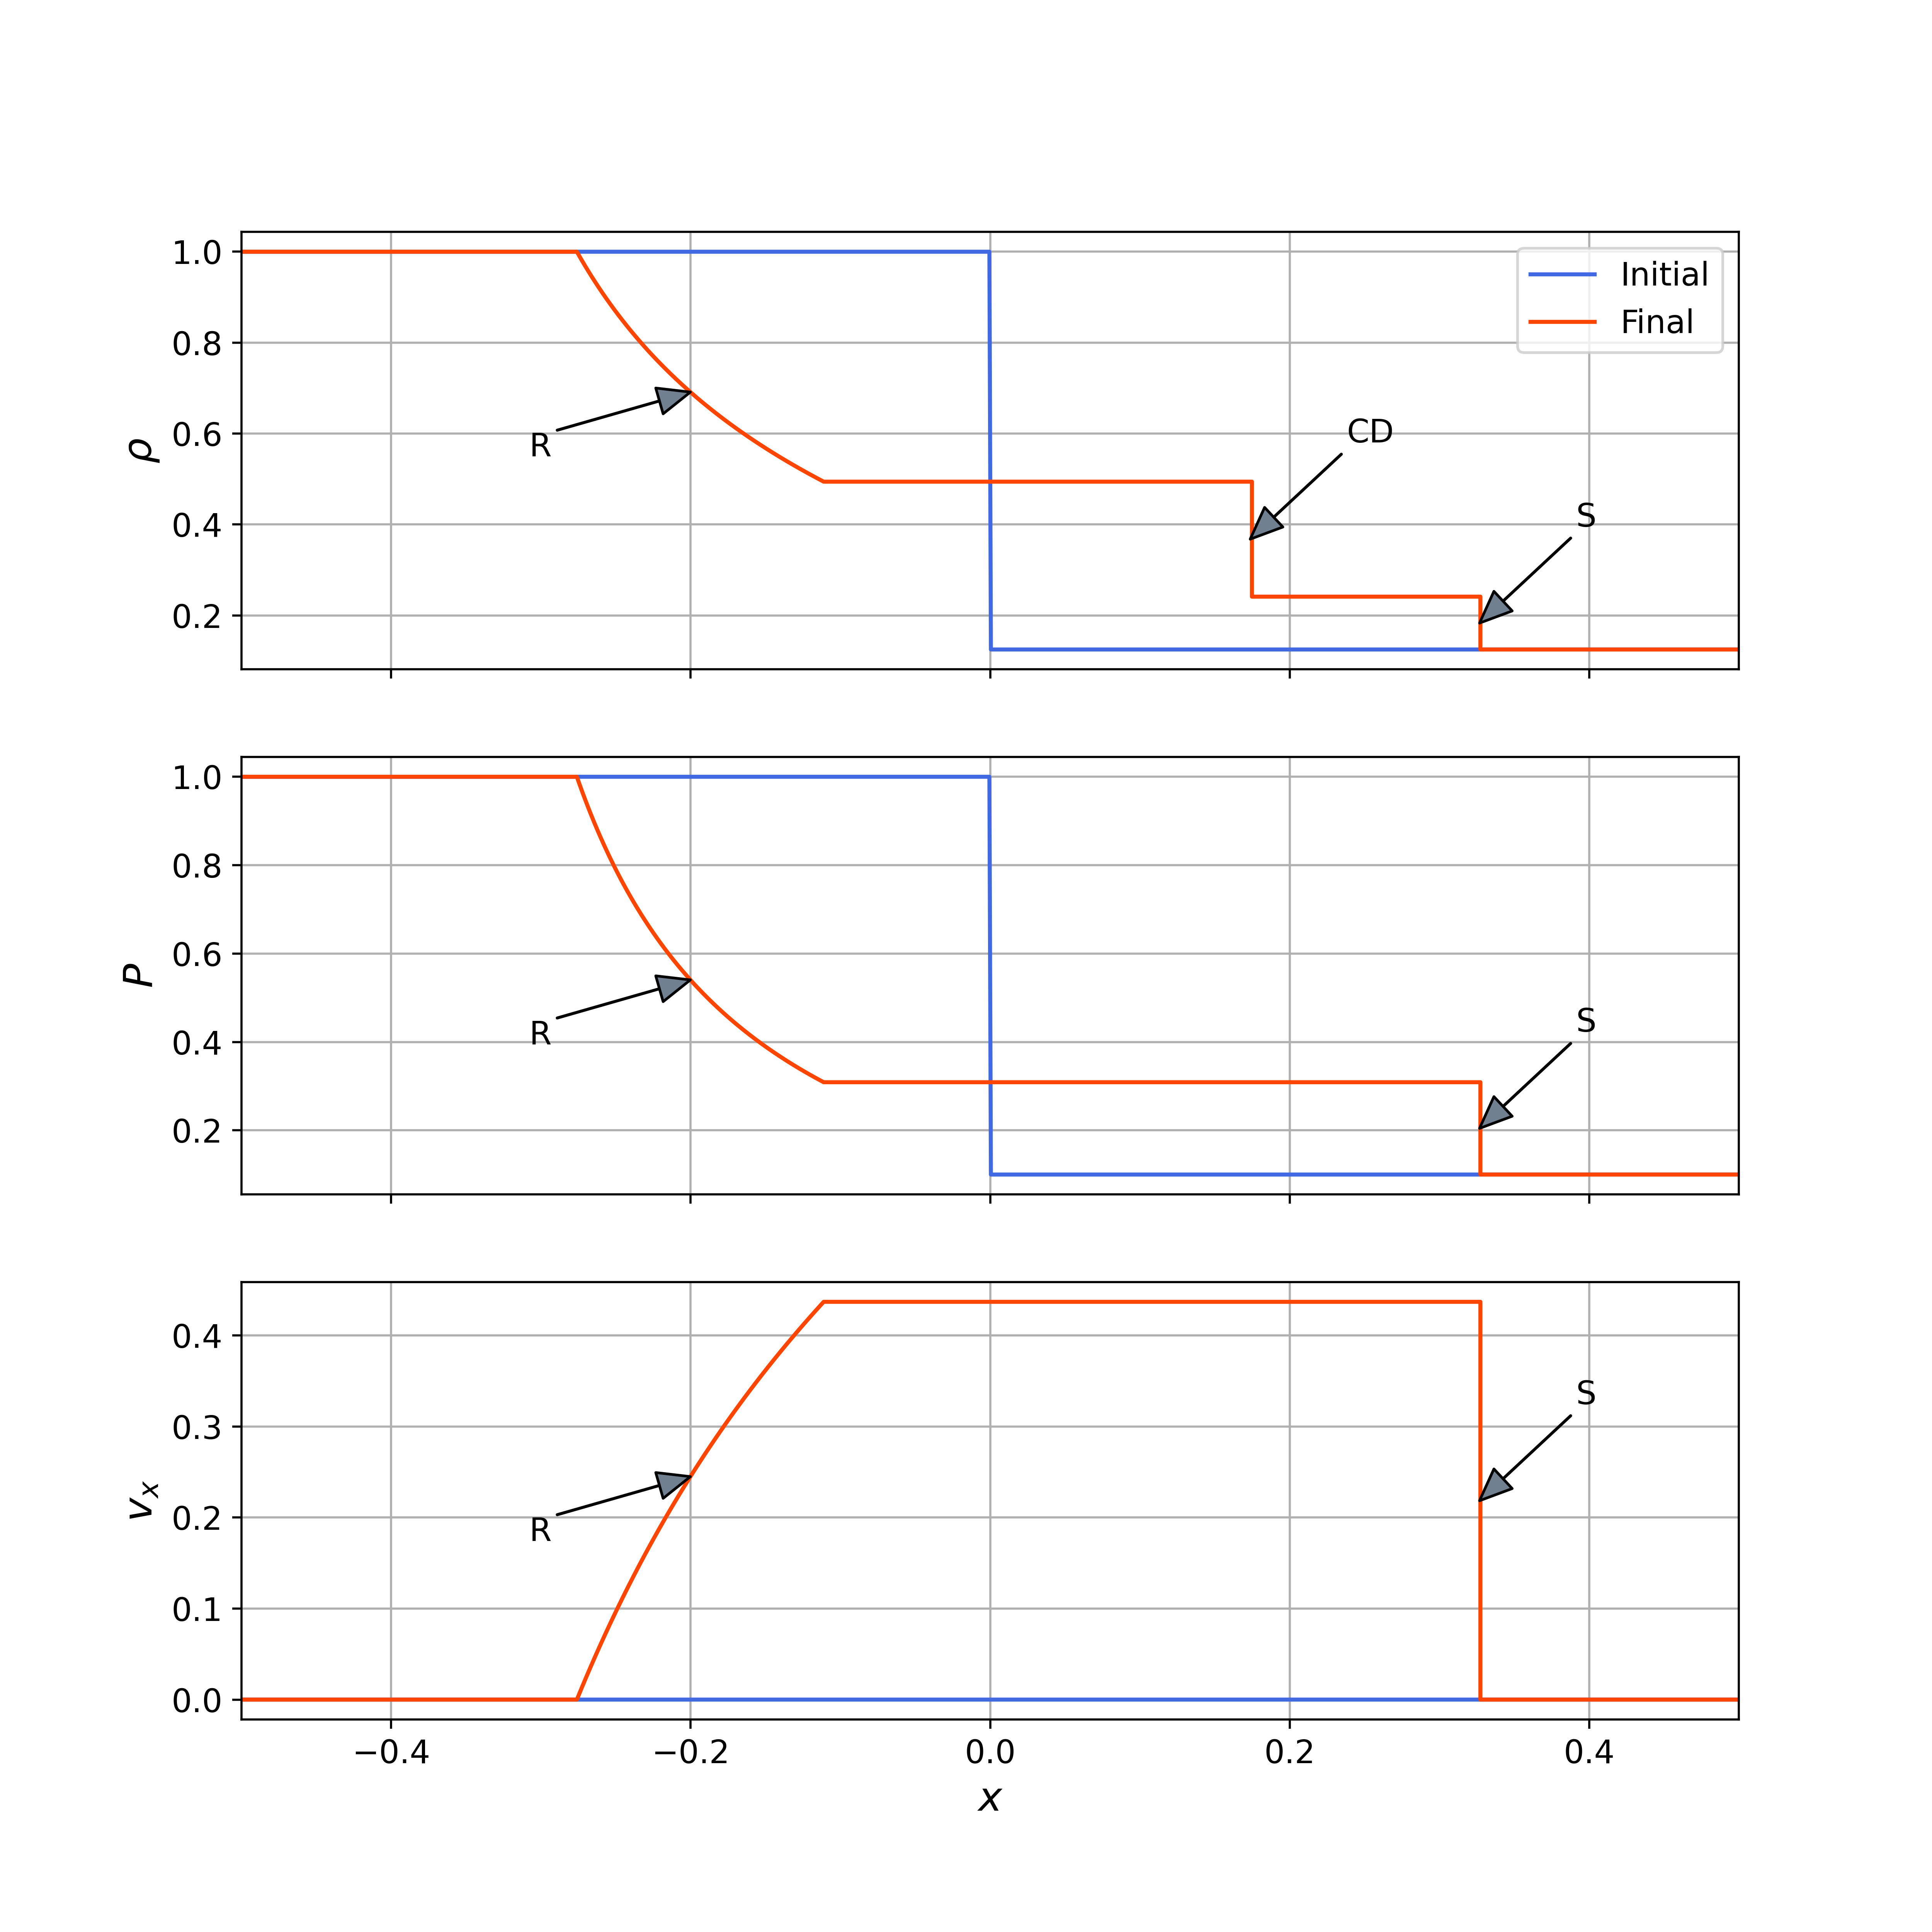
\includegraphics[width=1\linewidth]{images/all_exact_if.png}
    \captionof{figure}{Exact Solution; \figifcap; The arrows points at the different types of waves: R (Rarefaction), S (Shock) and CD (Contact Discontinuity).}
    \label{fig:all_exact_if}
\end{center}

\begin{center}
    \centering
    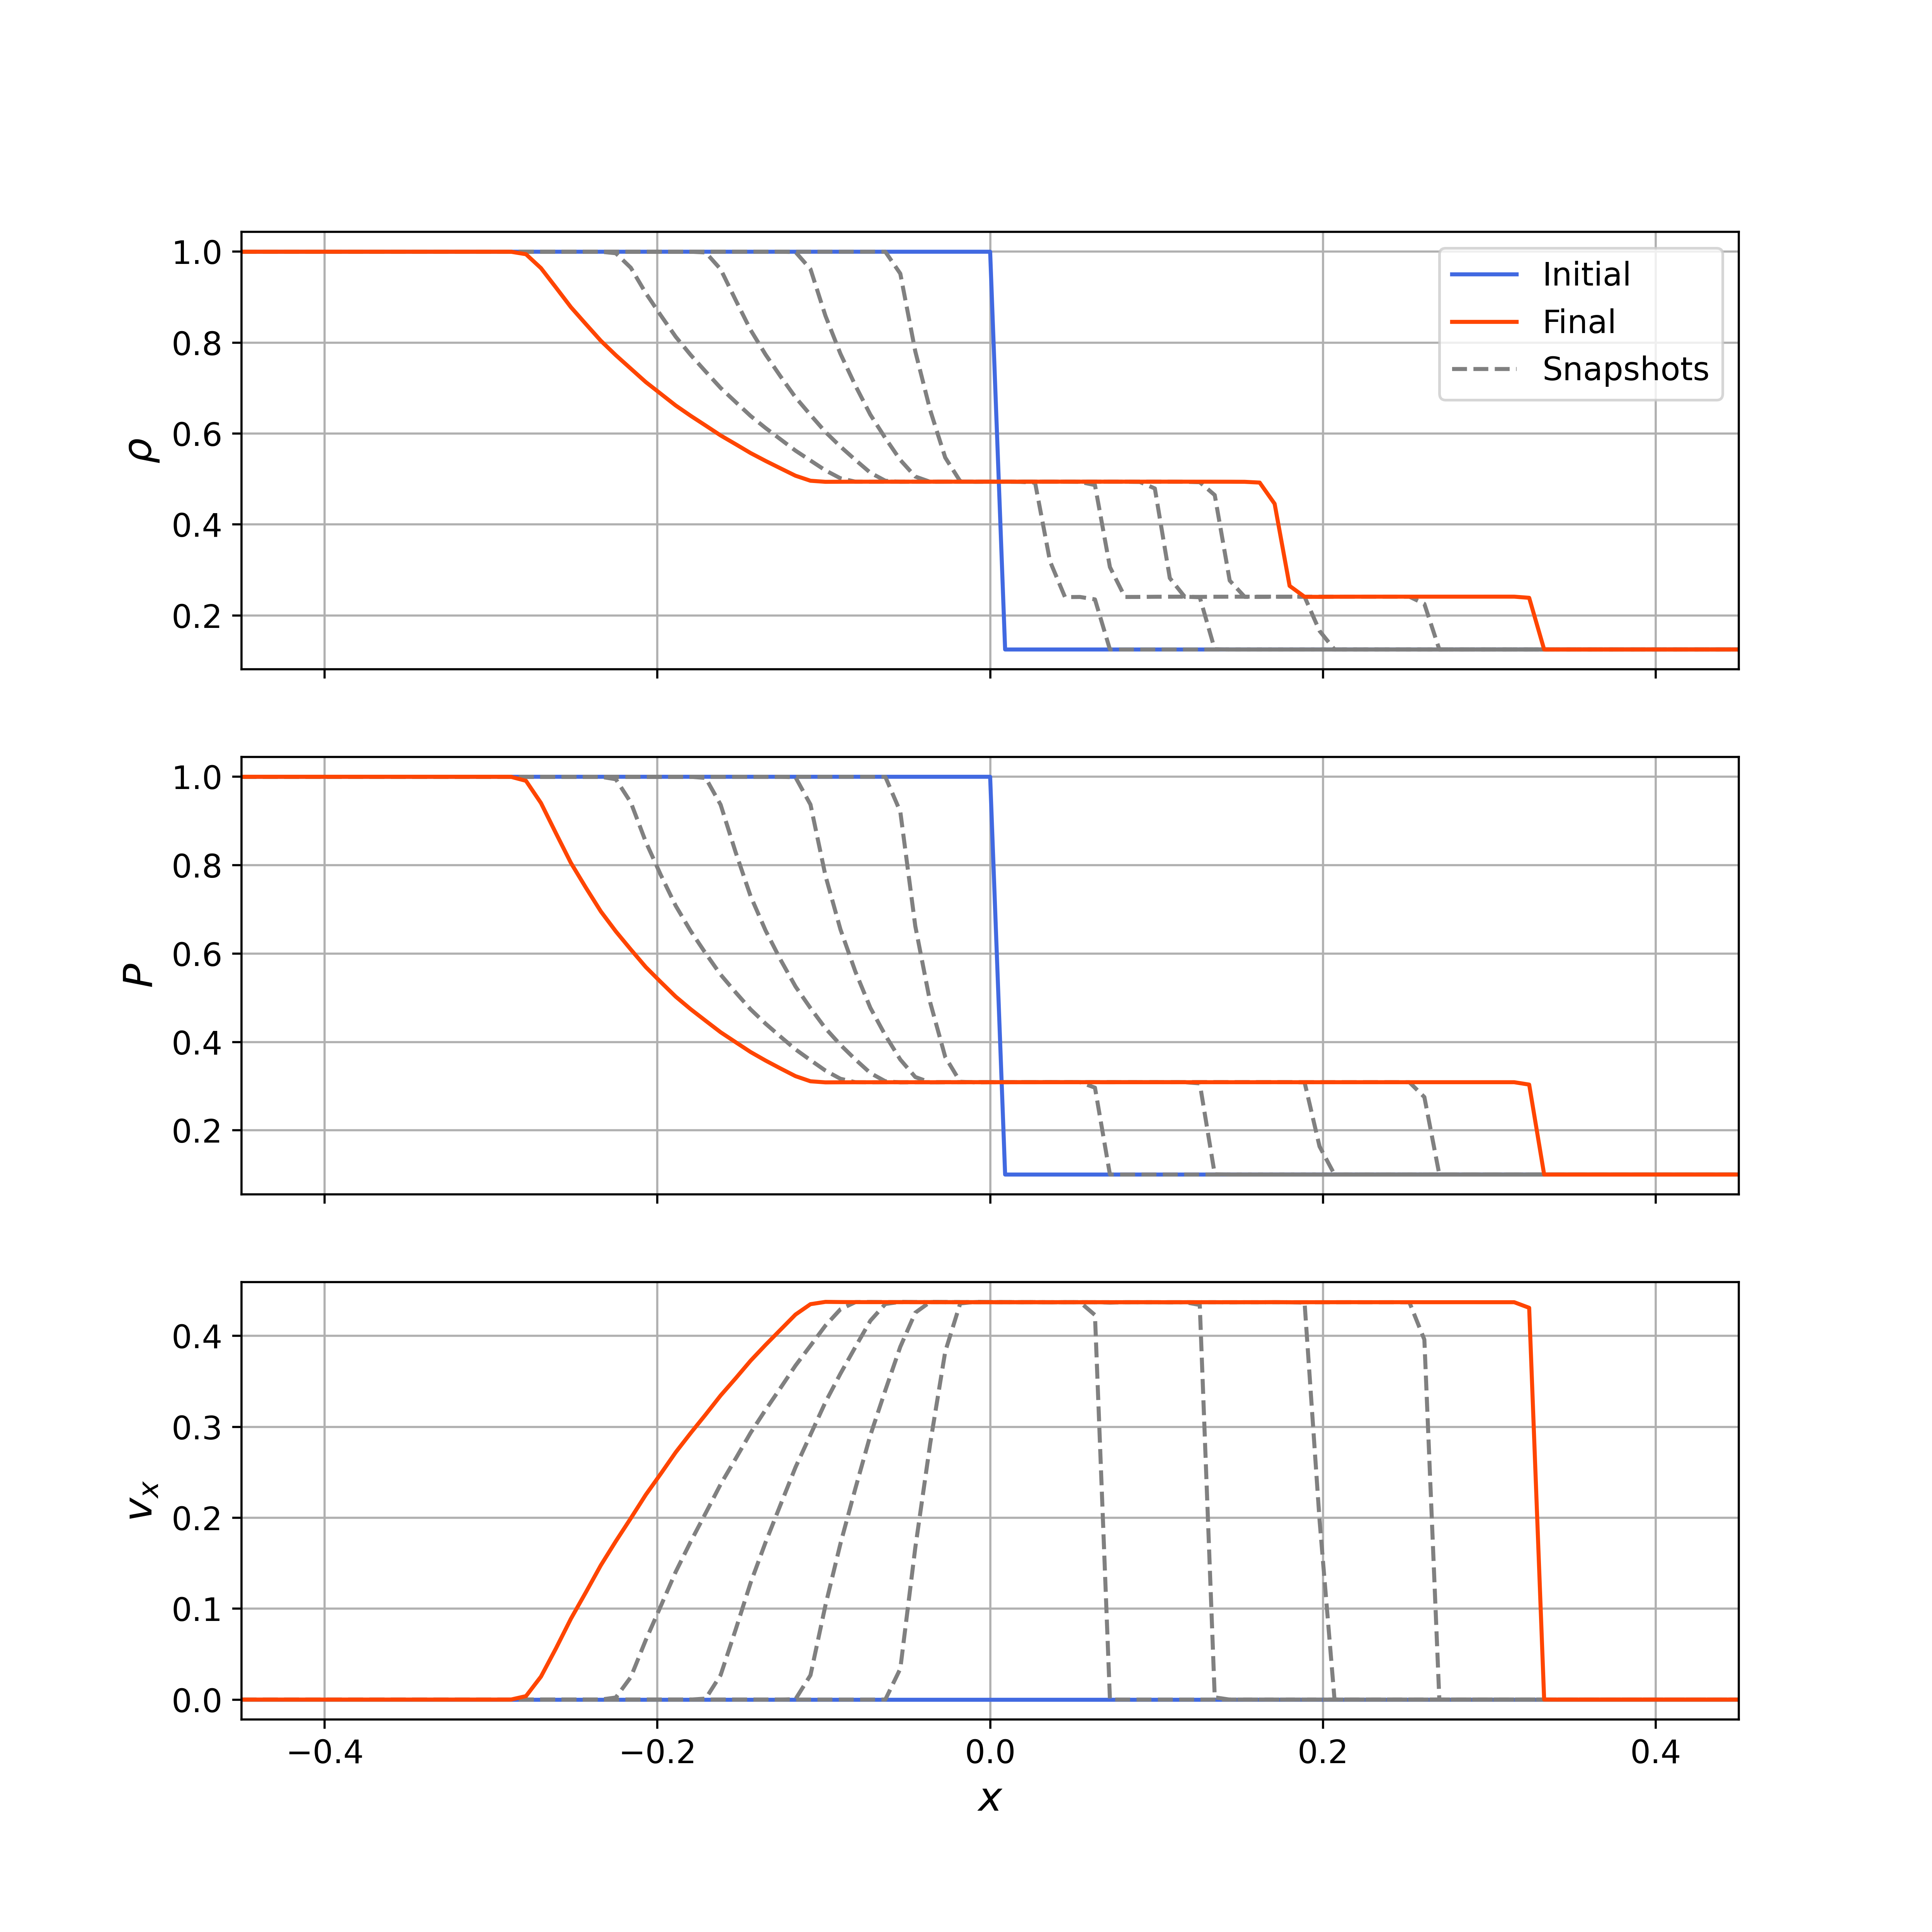
\includegraphics[width=1\linewidth]{images/all_1600_snapshots.png}
    \captionof{figure}{Numerical Solution; 1600 points; Snapshots.}
    \label{fig:all_1600_snapshots}
\end{center}

\begin{center}
    \centering
    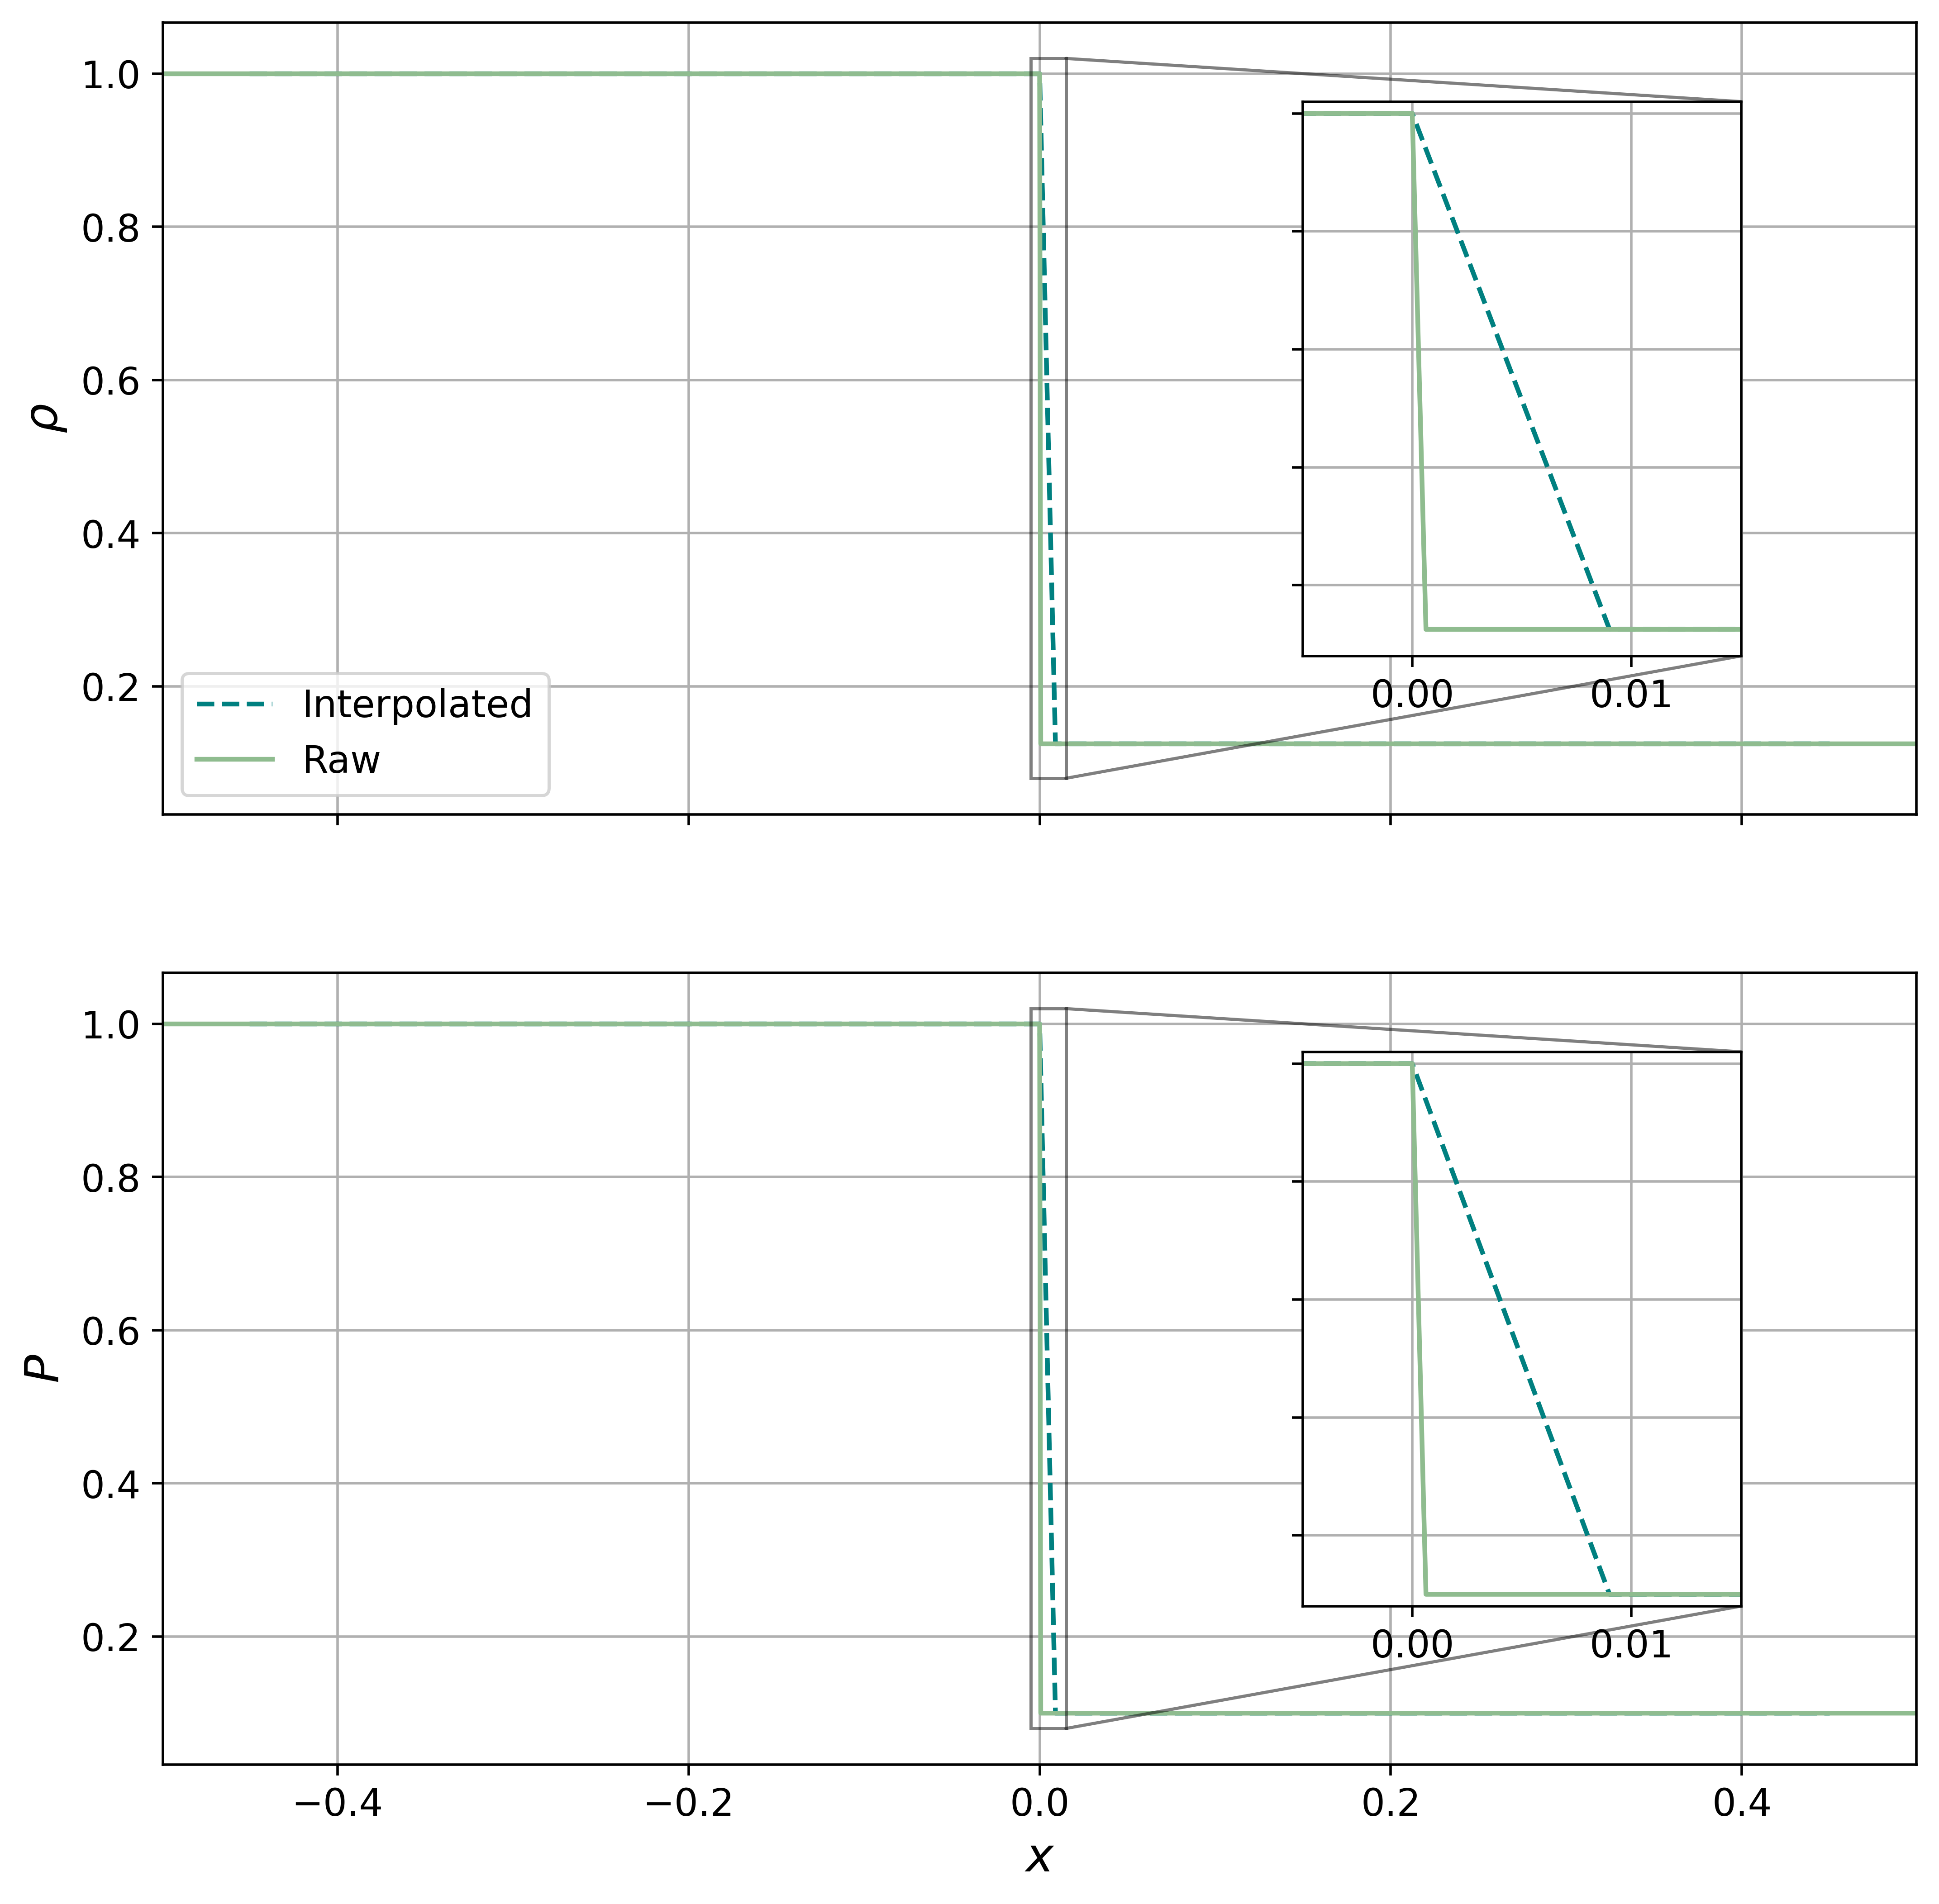
\includegraphics[width=1\linewidth]{images/all_1600_initial_compare.png}
    \captionof{figure}{Initial data; 1600 points; Raw and interpolated.}
    \label{fig:all_1600_initial_compare}
\end{center}

\begin{center}
    \centering
    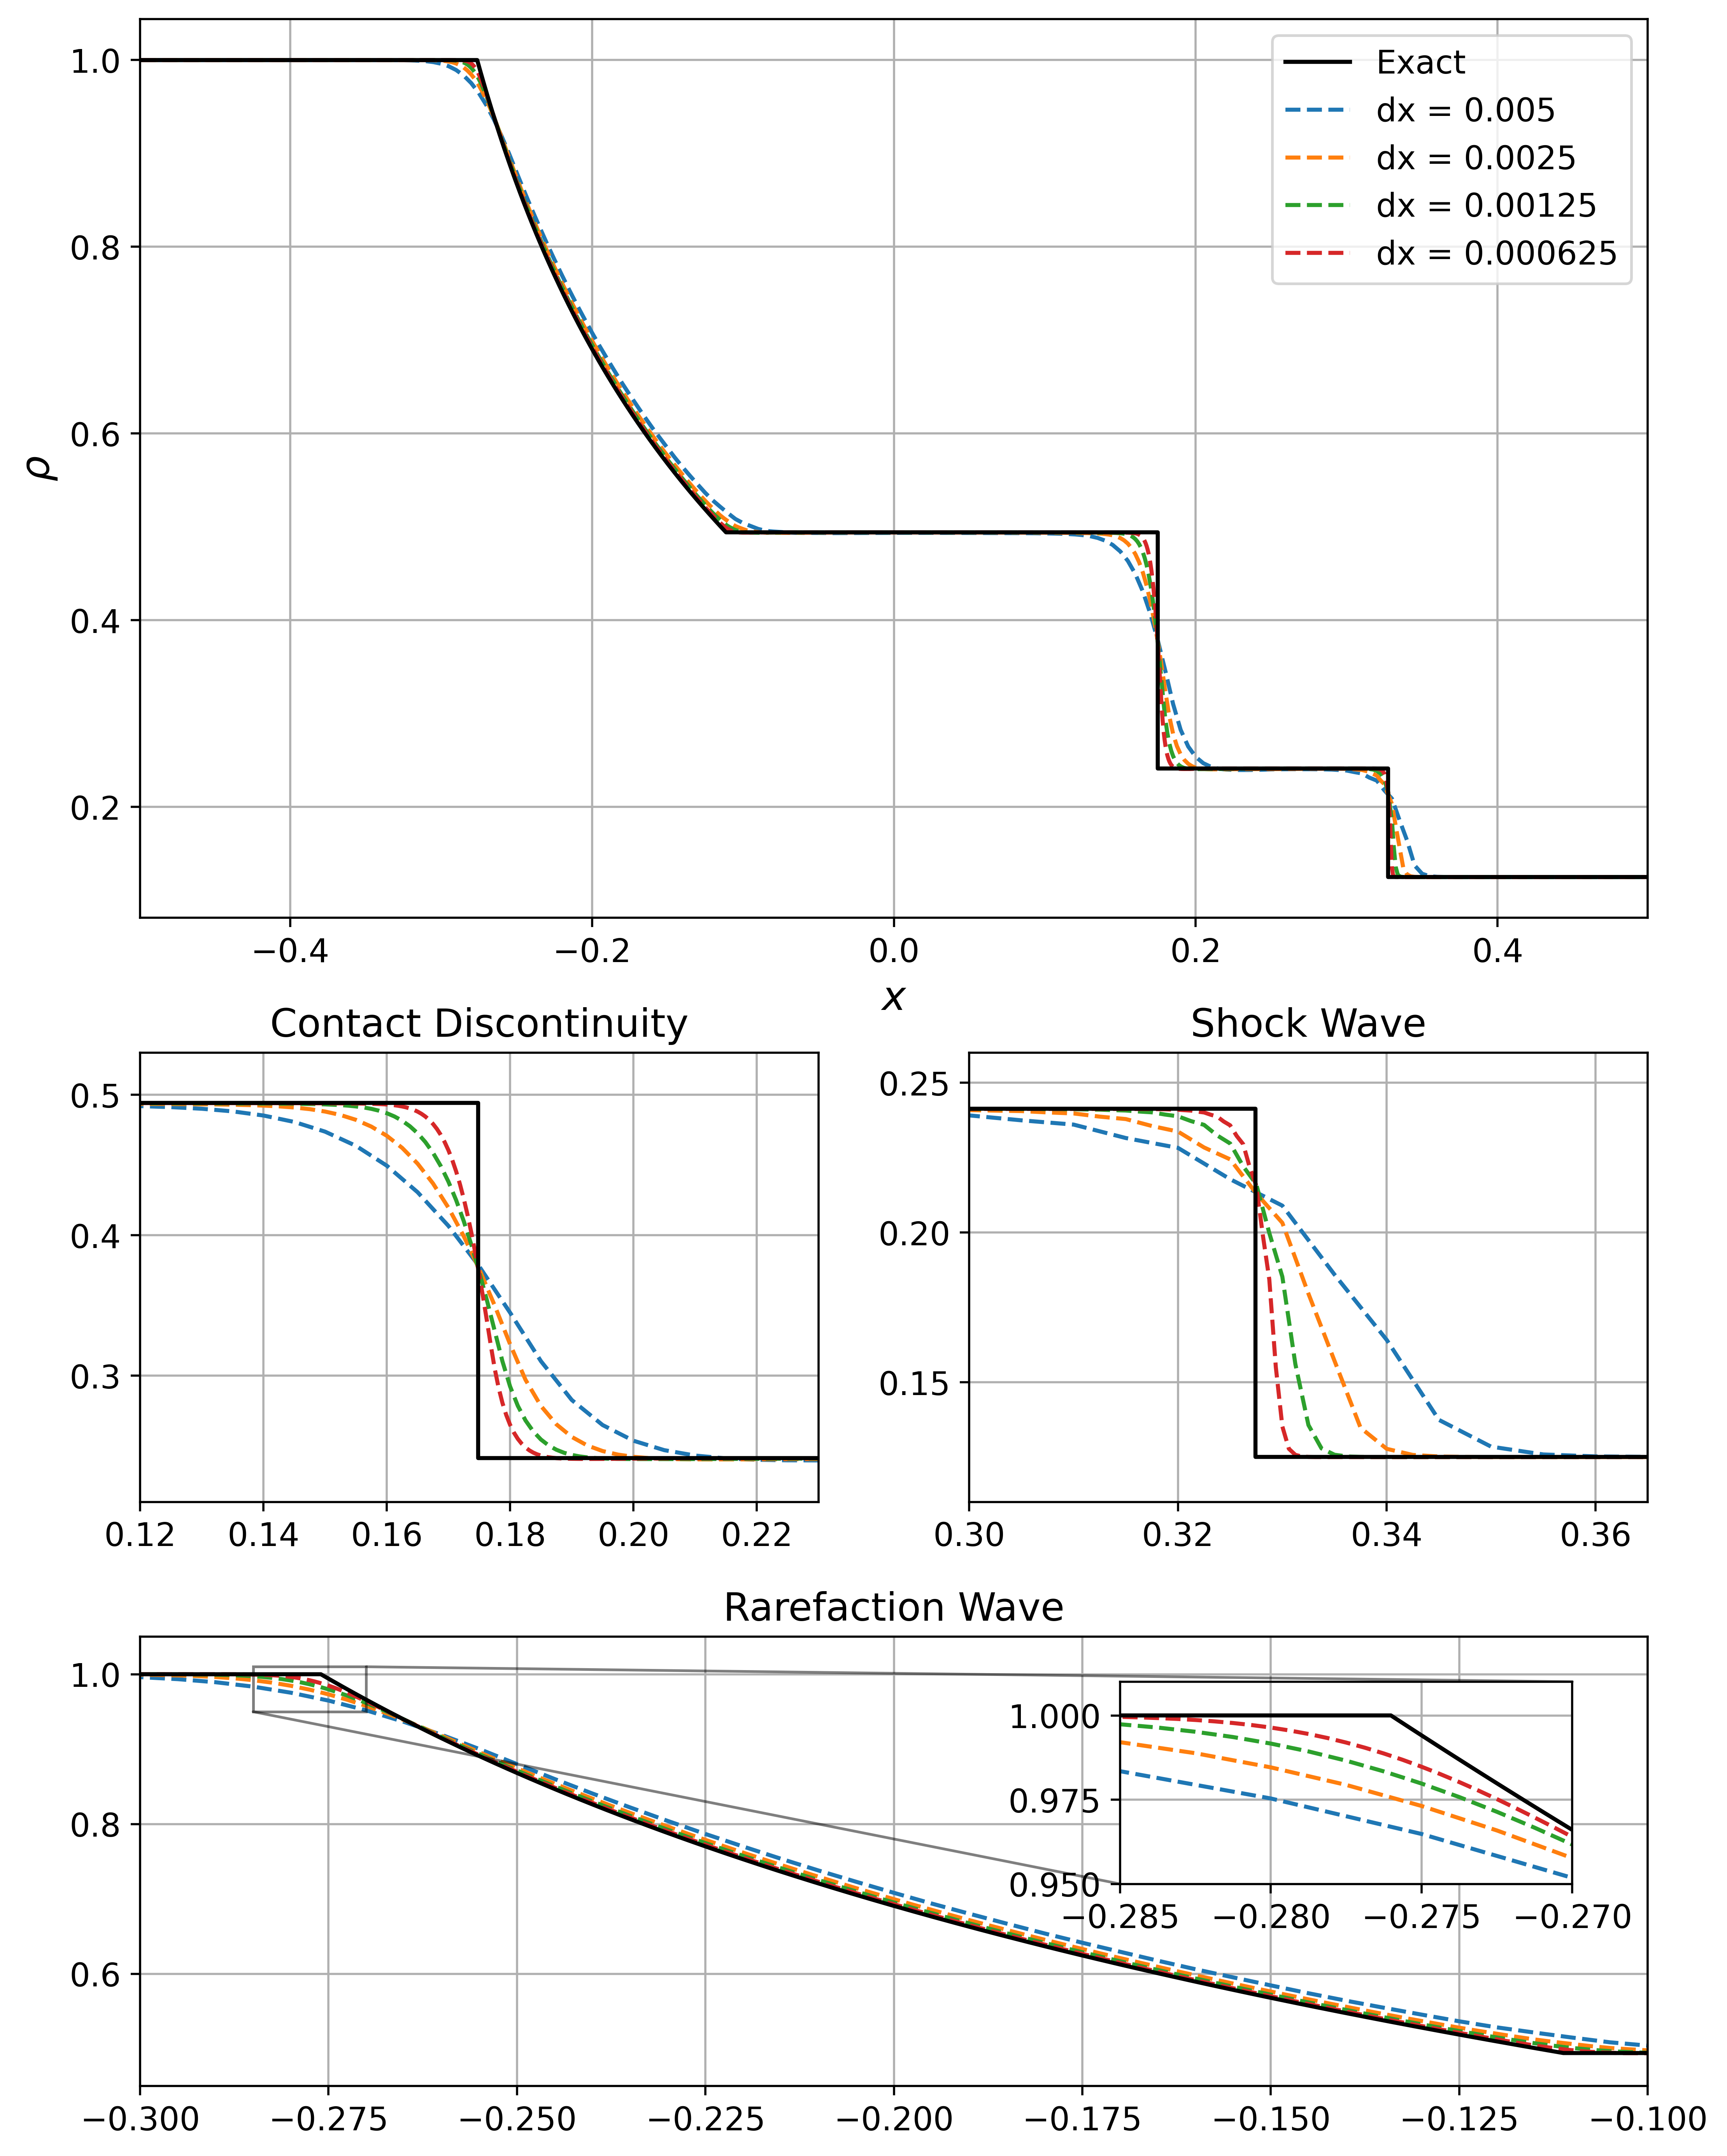
\includegraphics[width=1\linewidth]{images/rho_final_rescompare_raw.png}
    \captionof{figure}{Density; Final data; \figrescompcap.}
    \label{fig:rho_final_rescompare}
\end{center}

\begin{center}
    \centering
    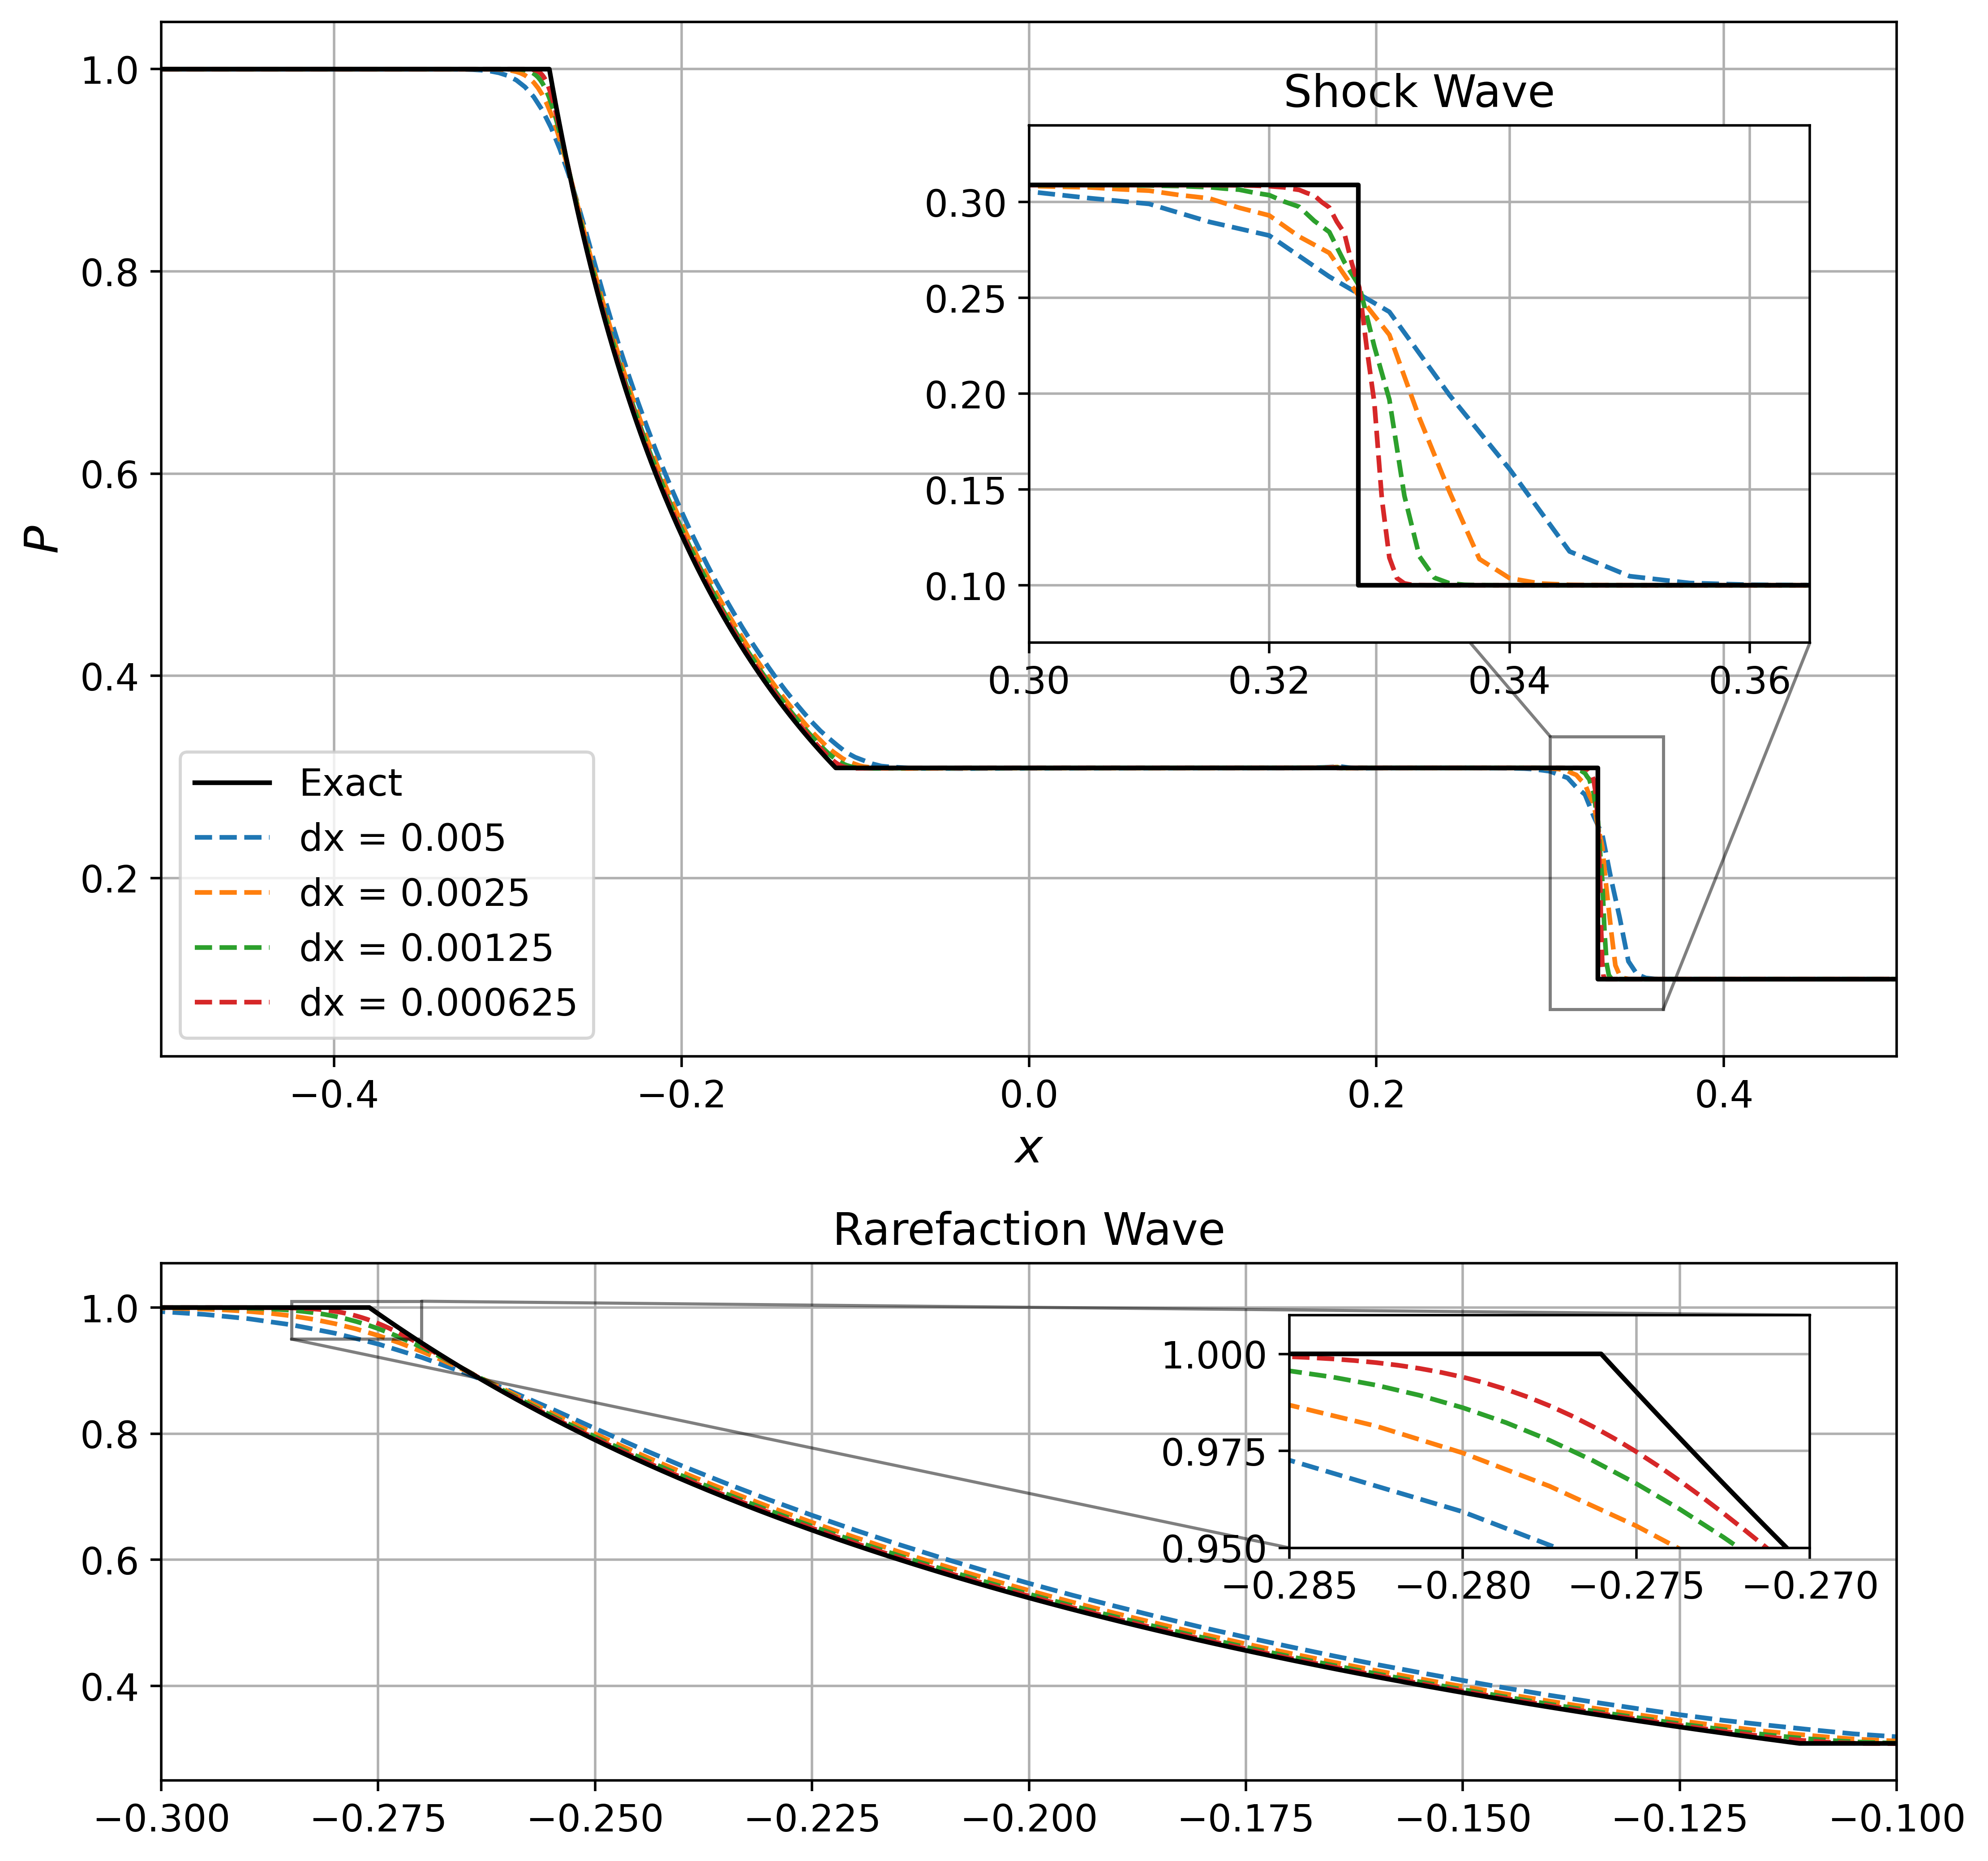
\includegraphics[width=1\linewidth]{images/press_final_rescompare_raw.png}
    \captionof{figure}{Pressure; Final data; \figrescompcap.}
    \label{fig:press_final_rescompare}
\end{center}

\begin{center}
    \centering
    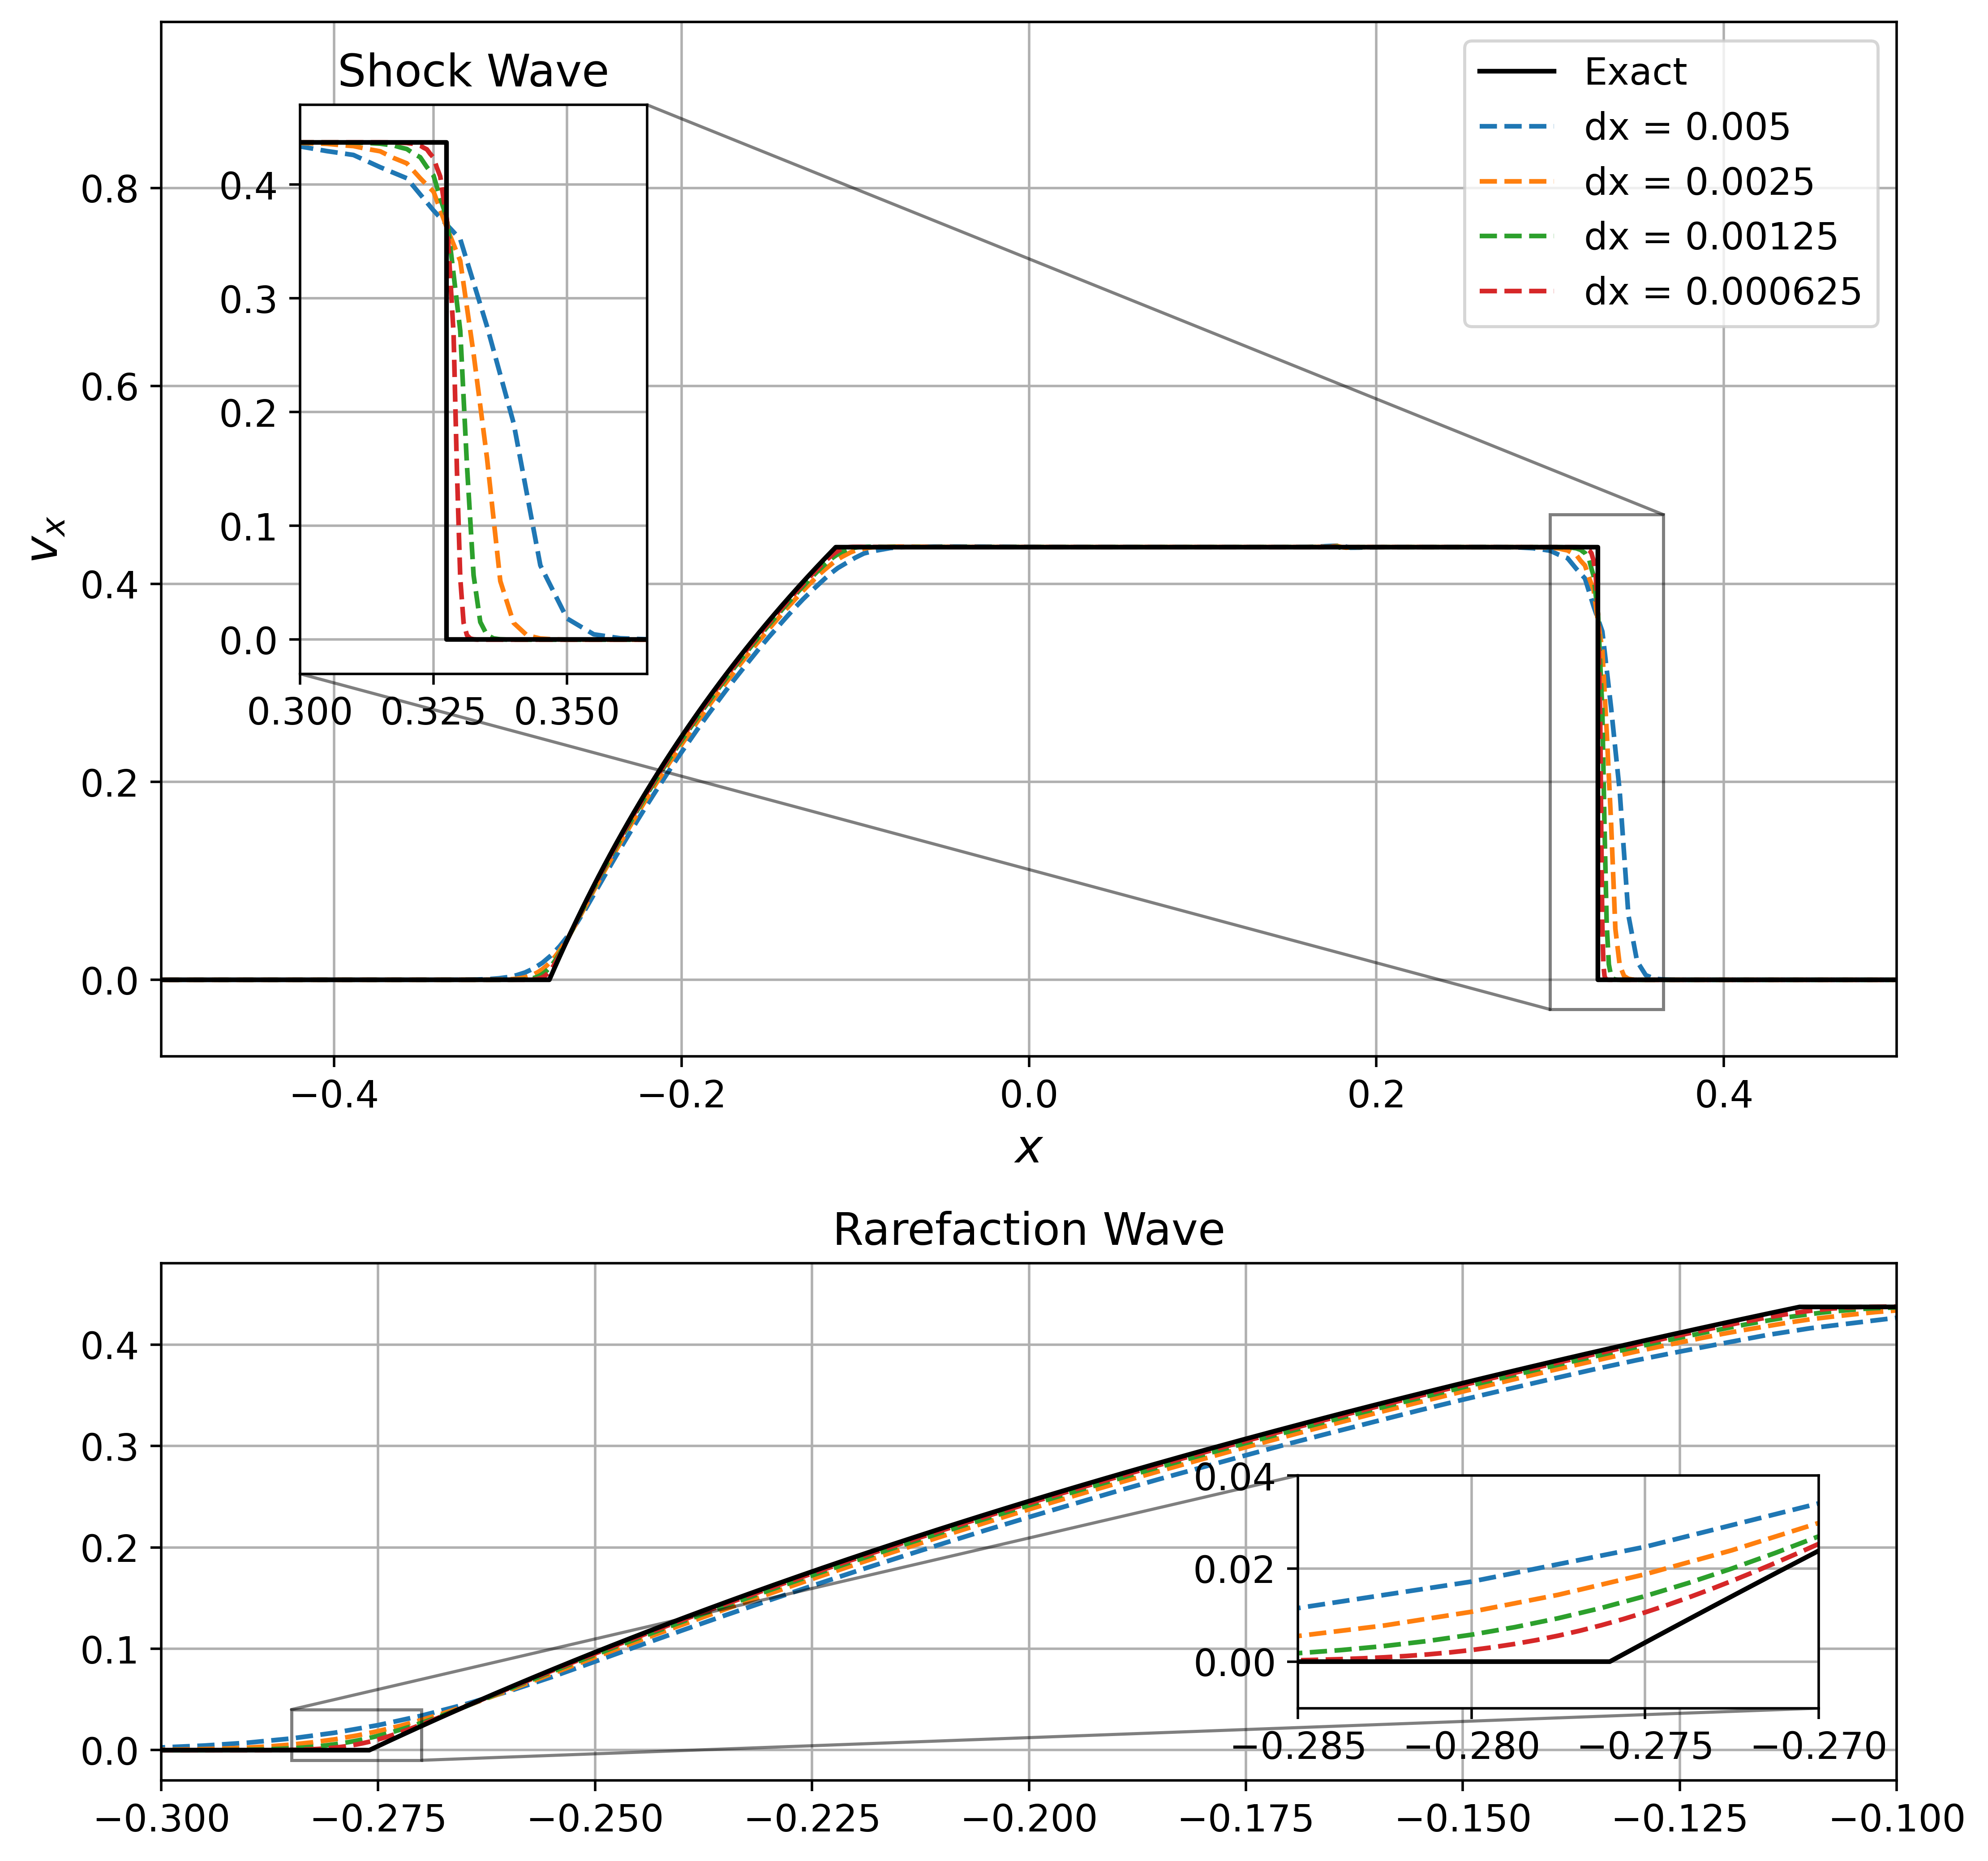
\includegraphics[width=1\linewidth]{images/vel[0]_final_rescompare_raw.png}
    \captionof{figure}{Velocity; Final data; \figrescompcap.}
    \label{fig:vel_final_rescompare}
\end{center}

\newpage

\section{TOV Evolution}

The \acrfull{tov} equation describes the physical properties of a spherically symmetric body in hydrostatic equilibrium under its own gravity. In this exercise, we study the evolution of the central value of the rest mass density (\(\rho_c\)) of a stable \acrfull{ns} using the \acrshort{etk}. The exercise is divided into two parts: in the first part, we evolve the system using different resolutions to study the numerical effects on the simulations; in the second part, we also introduce a pressure perturbation and analyze the response of the star.

The input and output of the thorns used for the evolution are in geometric units: \(G = c = M_\odot = 1\). We provide some conversion factors to convert from \acrfull{iu} to physical units for the variables we are interested in:

\begin{itemize}
    \item \textit{Length} from [\(\mathrm{M_\odot}\)] to \([\mathrm{km}]\): multiply by \(1.477\)
    \item \textit{Time} from [\(\mathrm{M_\odot}\)] to \([\mathrm{ms}]\): multiply by \(4.926 \times 10^{-3}\)
    \item \textit{Density} from [\(\mathrm{M_\odot^{-2}}\)] to \([\mathrm{g\ cm^{-3}}]\): multiply by \(6.176 \times 10^{17}\)
\end{itemize}

\noindent
In every part of the exercise, the final time of the simulation is set to \(400\ \mathrm{M_\odot}\) or about \(2\ \mathrm{ms}\). The \acrshort{ns} is centered at the origin of the reference frame, and the numerical grid spans in each direction the \([0, 24]\ \mathrm{M_\odot}\) interval, which corresponds roughly to a \(35\ \mathrm{km}\) side cube. The evolution of the equations in the regions of the stars outside of the grid domain is handled by the \textit{ReflectionSymmetry} thorn which mirrors the solution computed in the 3-dimensional \([0, 24]\) cube using the spherical symmetry of the problem. In every simulation, there is also one refinement level set on the \([0, 12]\ \mathrm{M_\odot}\) interval, having twice the starting resolution. For both parts of the exercise, a simulation has been run with each of the following grid spacing of the main grid in each of the three Cartesian directions: \(\{2.0, 1.0, 0.5\}\).

\subsection{Changing the resolution}

Figure \ref{fig:ns_rho_init_rescompare} shows the projection on the \(xy\) plane of the rest mass density of the initialized \acrshort{ns} with each of the used resolutions. The spherical symmetry of the problem is clearly broken by the discrete numerical grid we are using in the simulation. However, the higher the resolution, the better the star resembles a perfect sphere on the grid. This has direct effects on the numerical evolution of the \acrshort{ns}. Outside of the \acrshort{ns}, the value of the density is constant around \(10^{8}\ \mathrm{g\ cm^{-3}}\). This is because its minimum value has been manually set to \(10^{-10}\ \mathrm{M_\odot^{-2}}\) in the parameter file to prevent a transition to near-zero densities at the border of the star. Such a transition is undesirable from a numerical point of view because of the finite precision of the machine running the simulation.

Figure \ref{fig:ns_rhoc_0_rescompare} shows the evolution in time of the central value of the density with the used resolutions. Since no physical dissipation effect is taken into account in the simulation, if the spherical symmetry of the problem were preserved, then we'd expect the central density to stay constant in time. However, the fact that the star is discretized on the grid leads to the oscillations we observe. The lower the resolution, the further the star is from spherical symmetry, the greater the oscillations it experiences to adapt to the discretized space it lies in.

\subsection{Pressure perturbation}

In the second part of the exercise, we introduced a pressure perturbation in the evolving \acrshort{ns} by modifying the \textit{poly\_k} parameter of the \textit{EOS\_Omni} thorn. This means modifying the \(K\) coefficient in the polytropic \acrfull{eos} (Equation \ref{eq:poly_eos}) used to evolve the \acrshort{tov} solution:

\begin{equation} \label{eq:poly_eos}
    p = K \rho^\gamma
\end{equation}

\noindent
where \(K\) is the polytropic constant, and \(\gamma\) is the adiabatic index. The \acrlong{ns} has been initialized using \(K = 100\), while the \acrshort{eos} for the evolution has \(K = 110\). The simulations have been run using the same resolutions as before and the initial conditions are also unchanged (same as Figure \ref{fig:ns_rho_init_rescompare}).

Figure \ref{fig:ns_rhoc_pert_110_rescompare} shows the time evolution of the central density for the used grid spacings. The introduction of a pressure perturbation modifies the hydrostatic equilibrium of the \acrshort{ns}; the star tries to regain equilibrium, resulting in radial pulsations proportional to the amplitude of the perturbation. Figure \ref{fig:ns_radial_pulsations} shows some snapshots of the matter distribution of the \acrshort{ns} during the simulation for the finest spacing used. As already mentioned, since the star matter is treated as a perfect fluid and the simulation doesn't take into account any dissipation effects, the amplitude of the oscillations should stay constant in time. This is not the case because of the discreteness of the numerical simulation. In fact, we notice some evident damping for the low resolution case, while it is much weaker when the resolution gets increased. The density perturbations visible in Figure \ref{fig:ns_radial_pulsations} are due to the fictitious fluid the \acrshort{ns} is embedded in as a result of the fixed minimum value of the rest mass density.

However, we point out that pure numerical oscillations in the perturbed case are a minor effect with respect to the physical ones. Figure \ref{fig:ns_rhoc_all_compare} shows the central density evolution for the perturbed and the unperturbed cases plotted together in terms of relative percentage variation from the initial value.

\newpage

\begin{center}
    \centering
    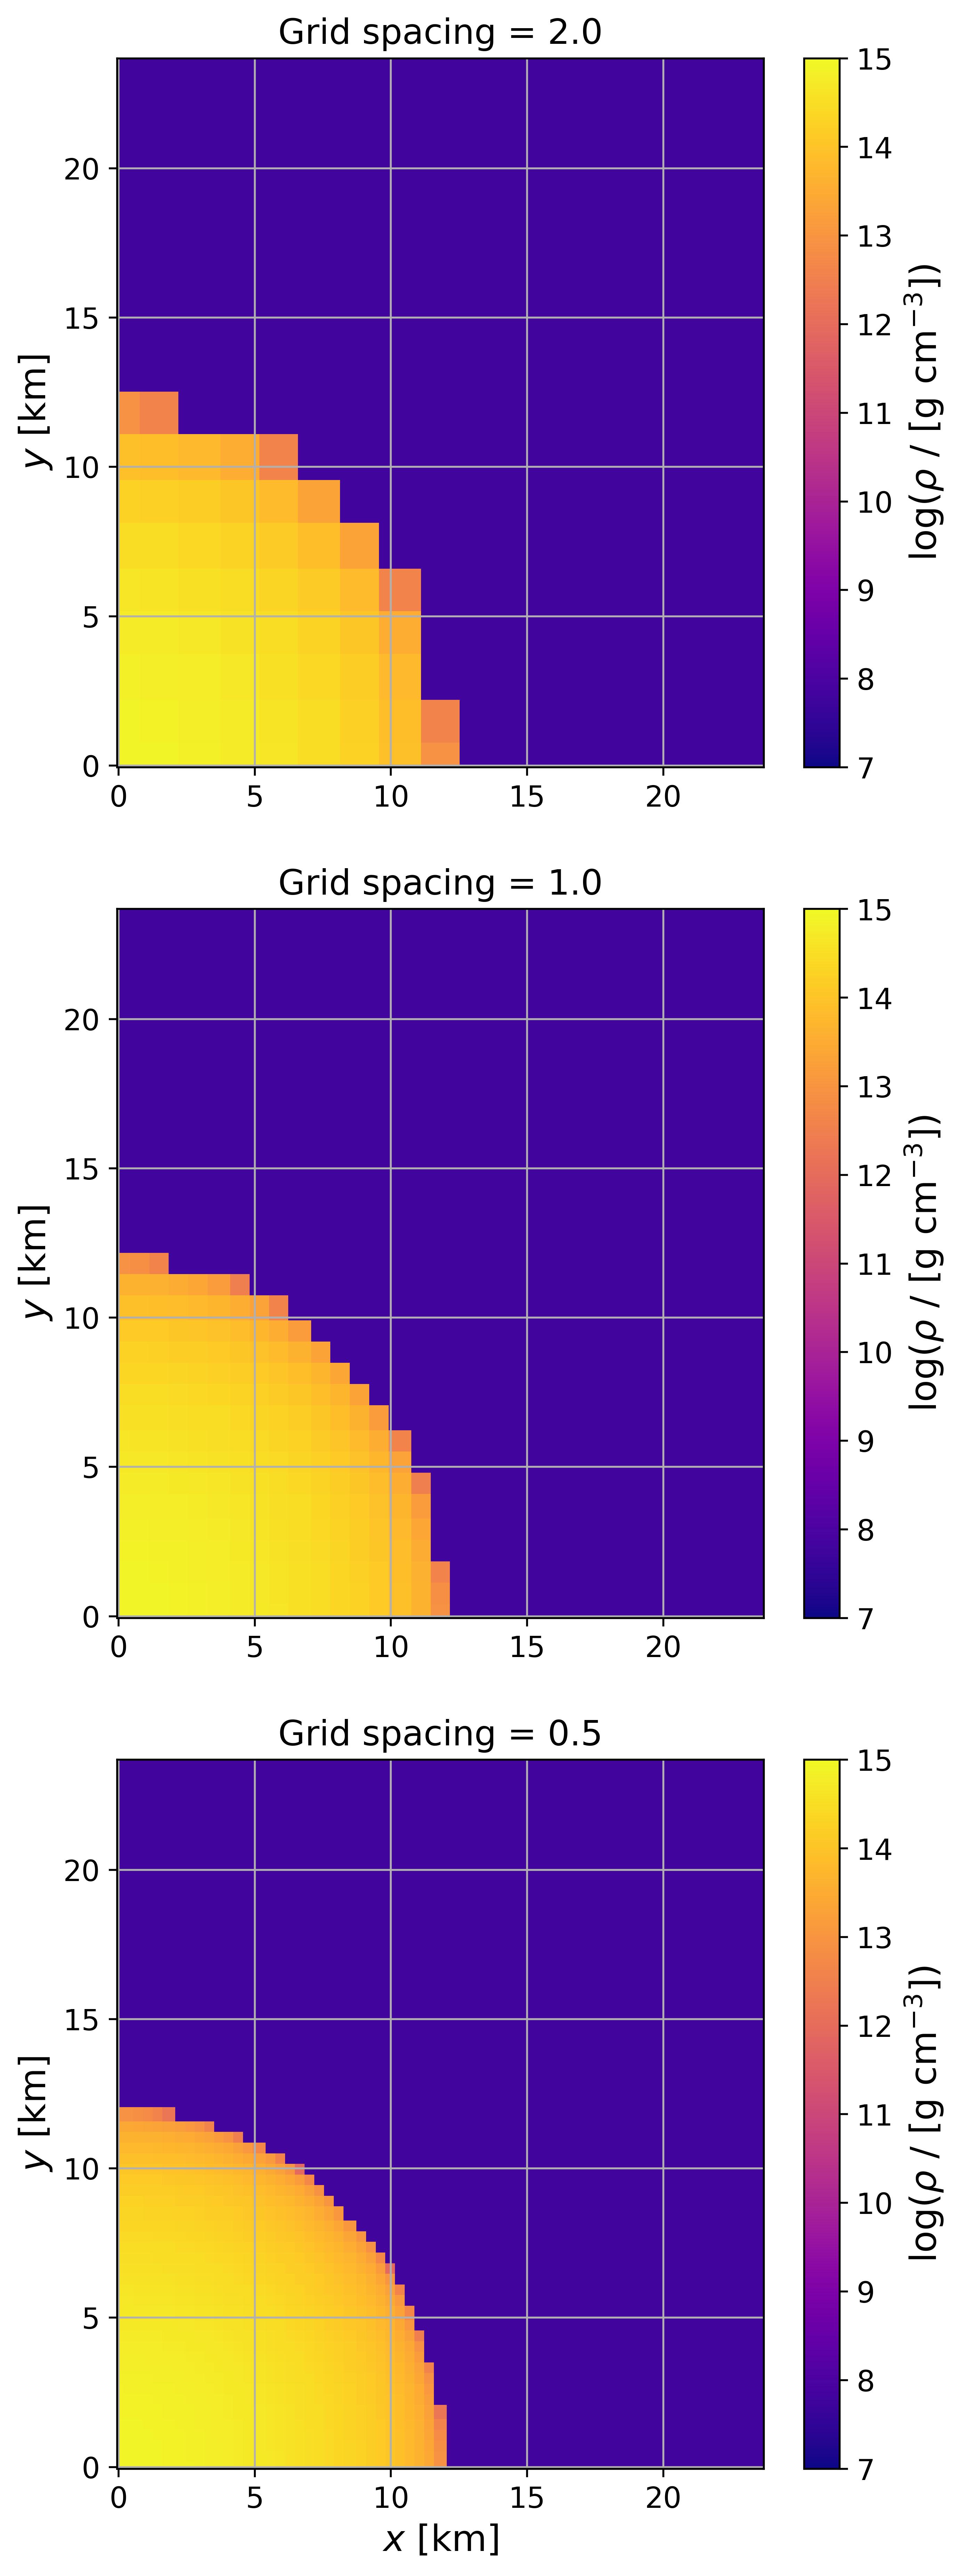
\includegraphics[height=0.9\textheight]{images/rho_init_rescompare.png}
    \captionof{figure}{Rest mass density; Initial data; \figrescompcap.}
    \label{fig:ns_rho_init_rescompare}
\end{center}

\begin{center}
    \centering
    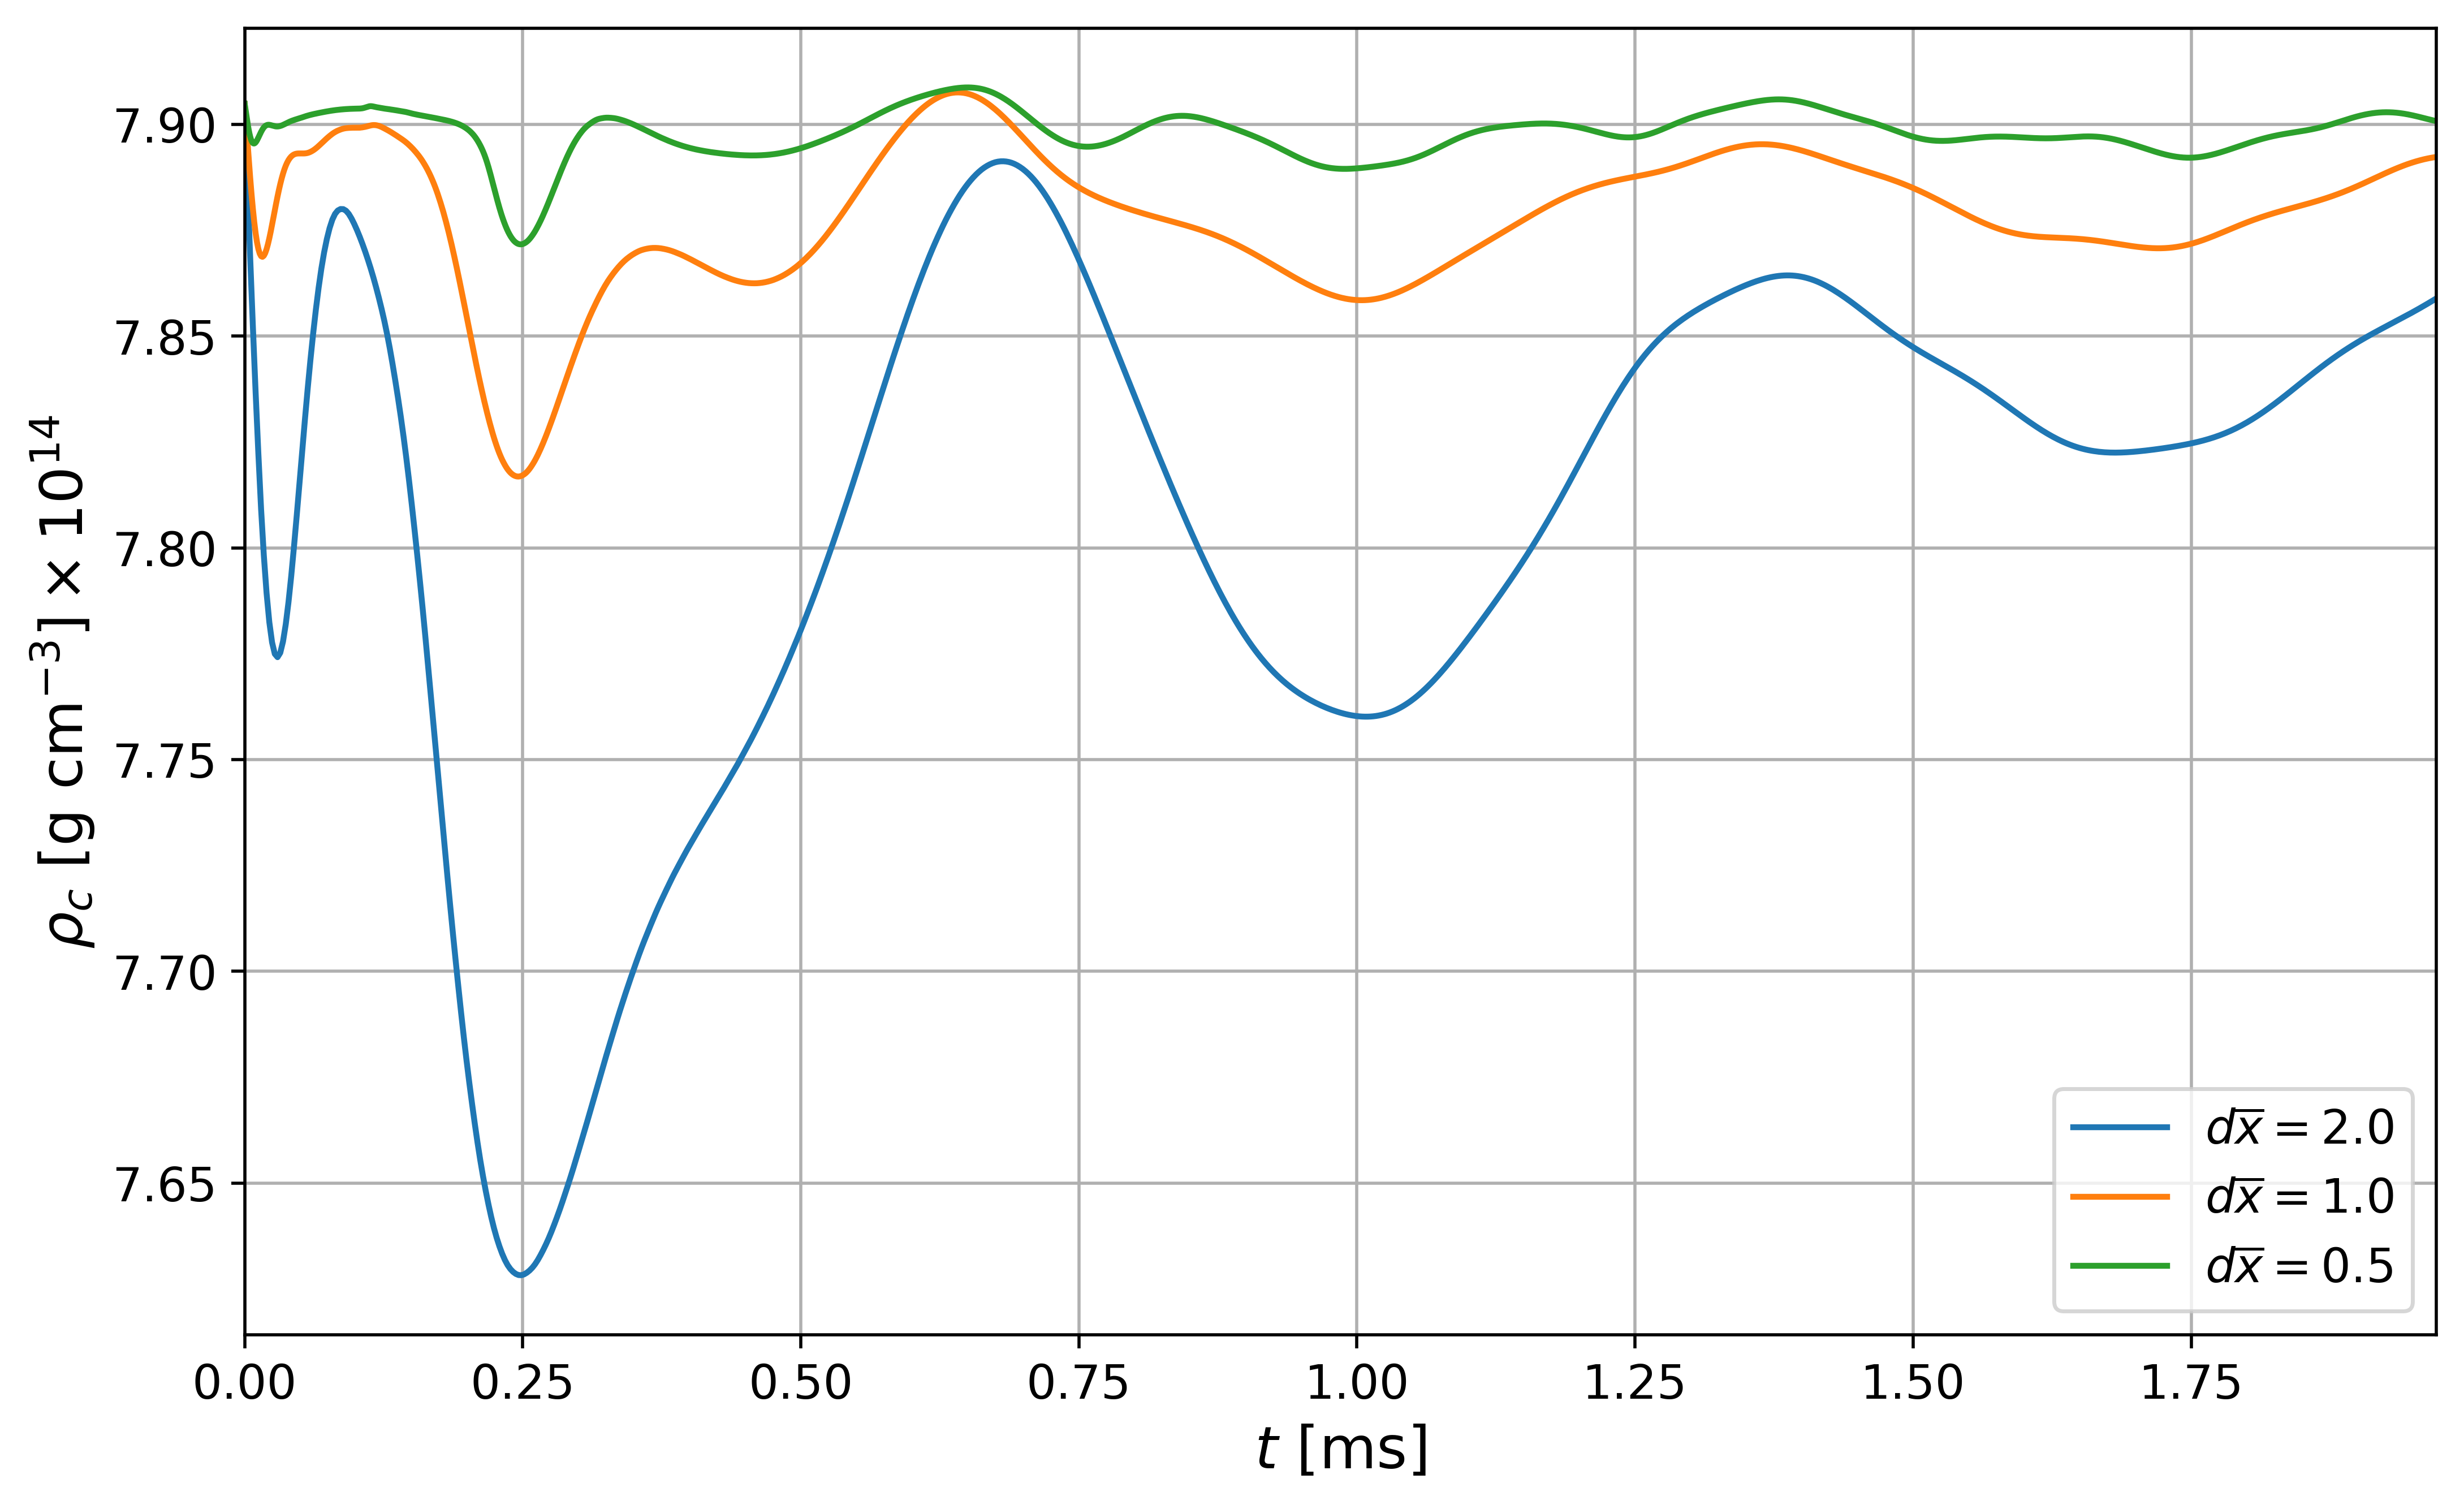
\includegraphics[width=1\linewidth]{images/rhoc_0_rescompare.png}
    \captionof{figure}{Unperturbed \acrshort{ns}; Central density; Time evolution; \figrescompcap.}
    \label{fig:ns_rhoc_0_rescompare}
\end{center}

\begin{center}
    \centering
    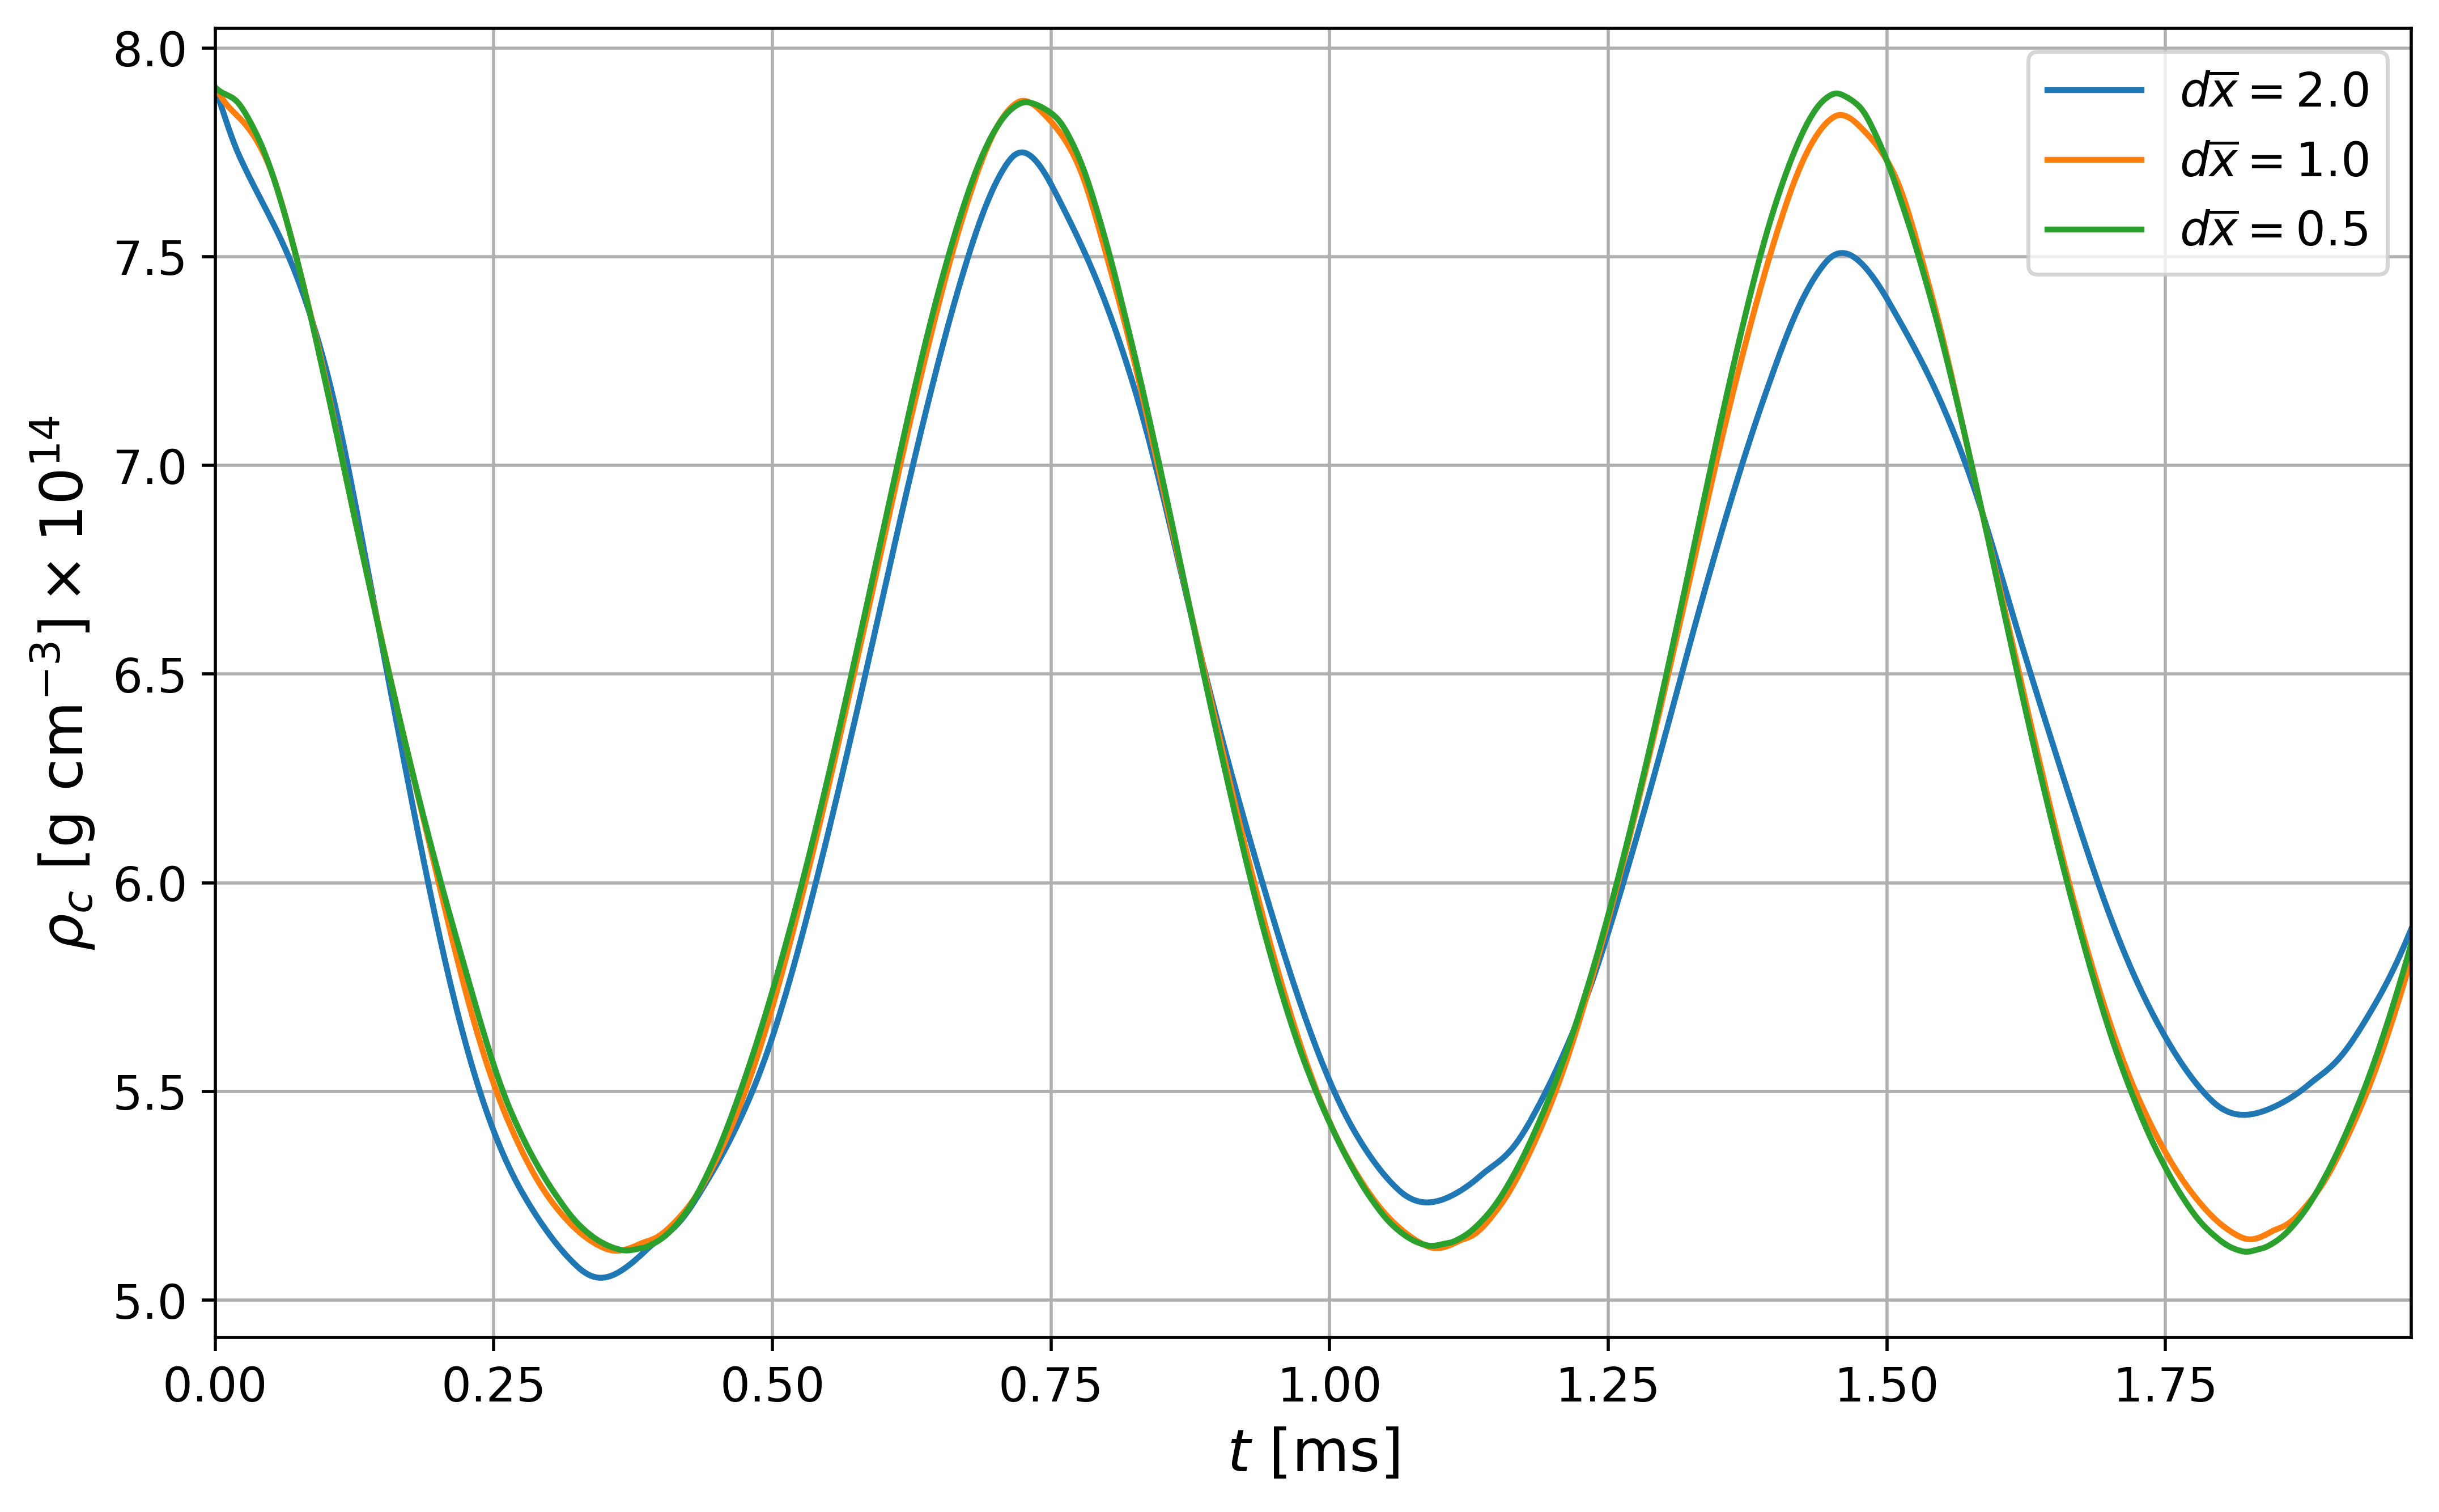
\includegraphics[width=1\linewidth]{images/rhoc_pert_rescompare.png}
    \captionof{figure}{Perturbed \acrshort{ns} (\(K = 110\)); Central density; Time evolution; \figrescompcap.}
    \label{fig:ns_rhoc_pert_110_rescompare}
\end{center}

\begin{center}
    \centering
    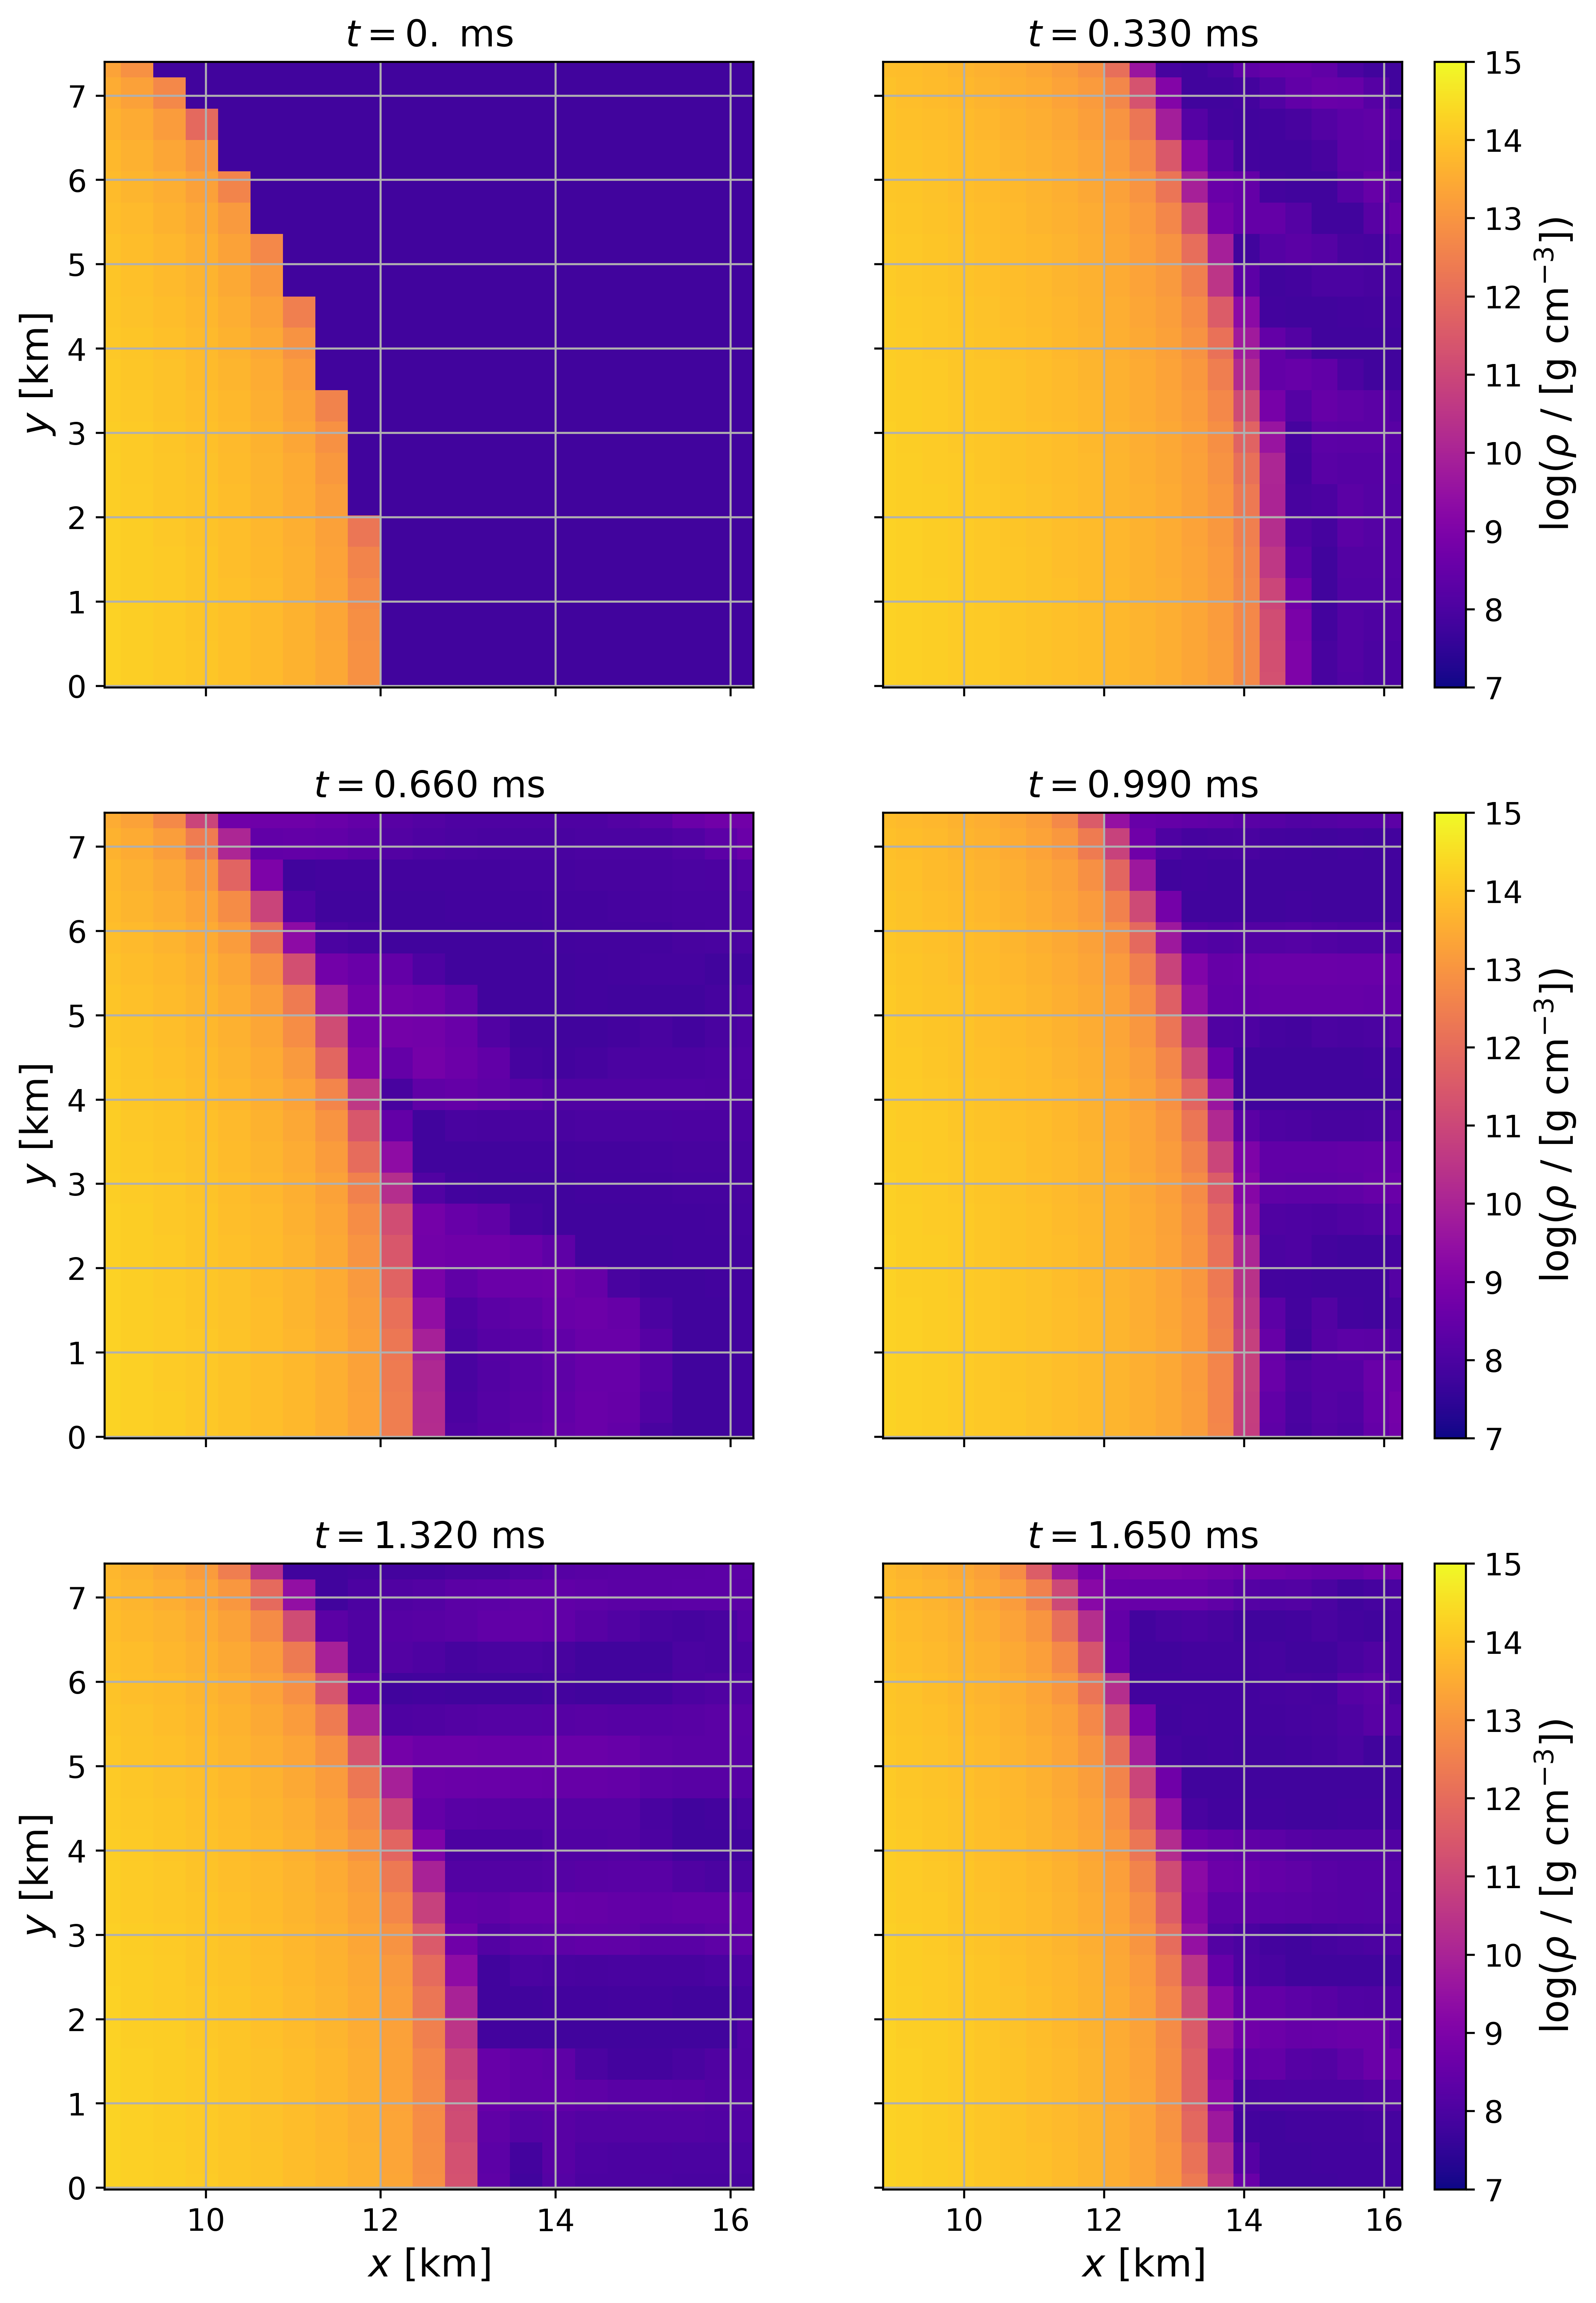
\includegraphics[height=0.9\textheight, width=1\textwidth, keepaspectratio]{images/rho_snapshots.png}
    \captionof{figure}{Perturbed \acrshort{ns} (\(K = 110\)); Rest mass density; Snapshots; Grid spacing = \(0.5\)}
    \label{fig:ns_radial_pulsations}
\end{center}

\begin{center}
    \centering
    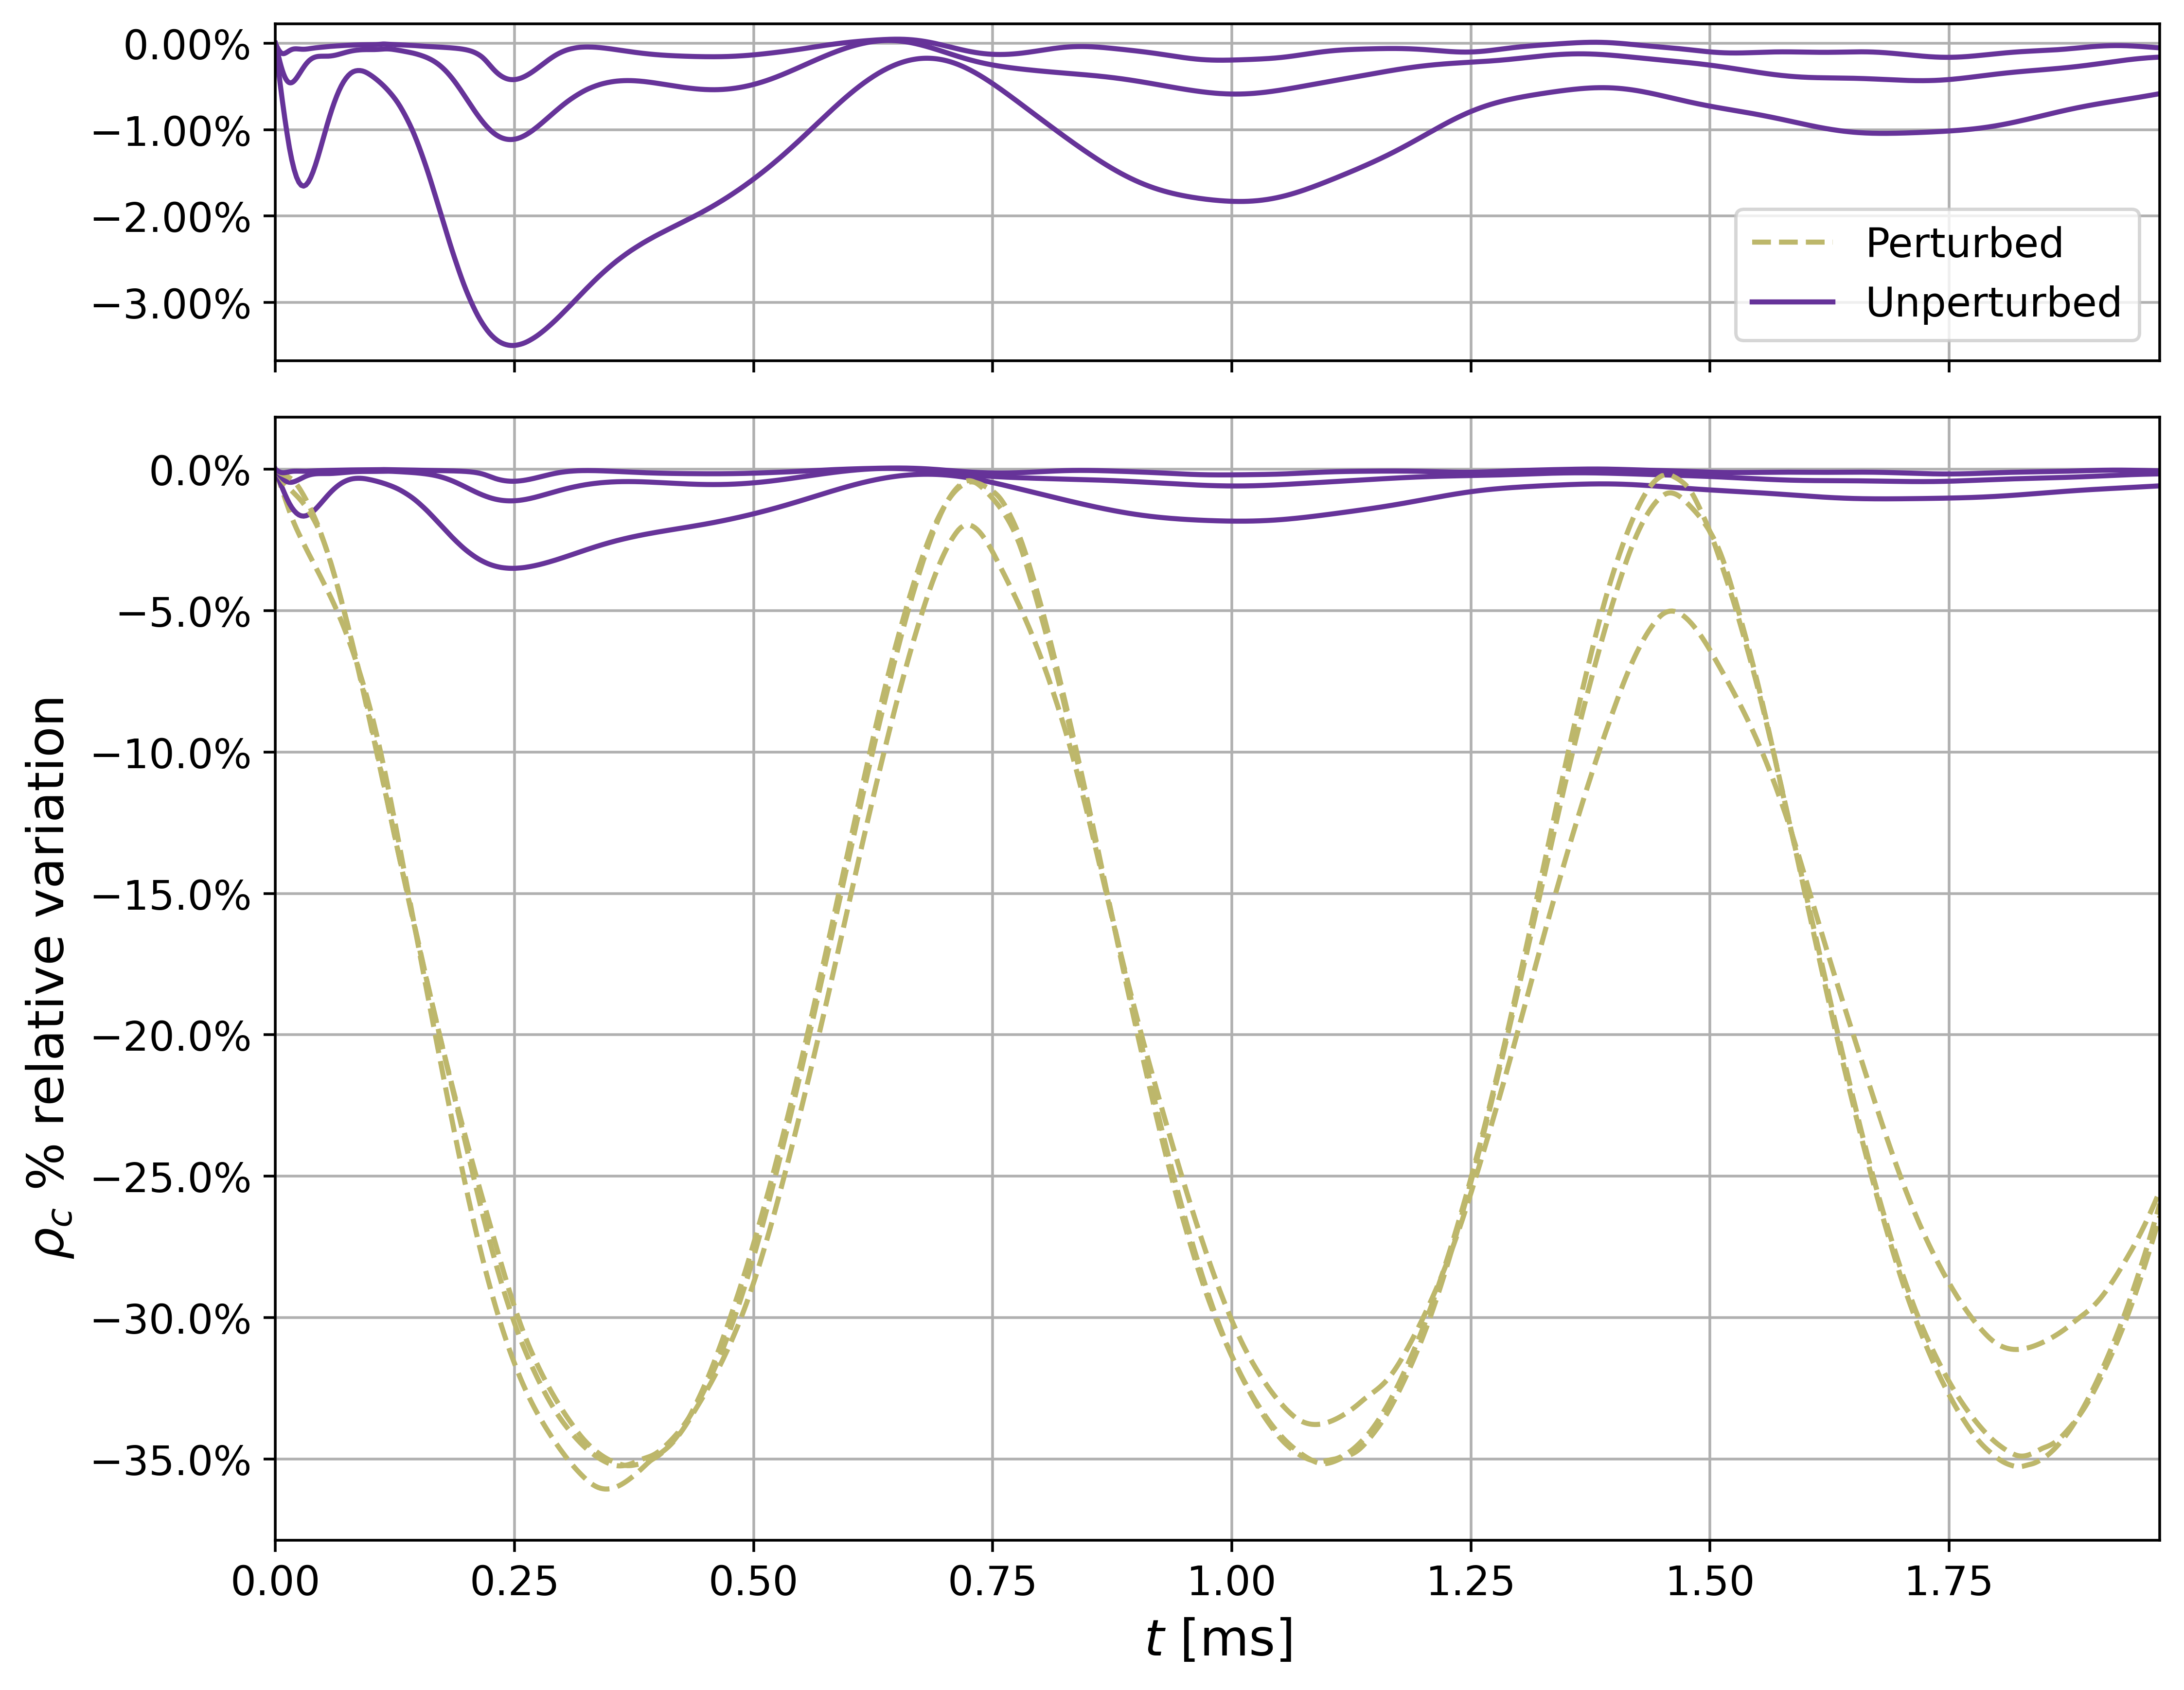
\includegraphics[width=1\linewidth]{images/rhoc_all_typecompare.png}
    \captionof{figure}{Central density; Time evolution; Comparison of perturbed and unperturbed case.}
    \label{fig:ns_rhoc_all_compare}
\end{center}

\newpage

\section{\acrlong{etk} parameters}

For the last exercise, we explain the meaning of some entries in the parameter files we used to run the simulations with the \acrlong{etk}.

\subsection{\acrfull{mol}}

The \acrlong{mol} is a way to convert a system of \acrfull{pdes} into a system of \acrfull{odes}. Then, given the separation of the time component and a way to discretize space, an \acrshort{ode} integrator can be used to perform the time evolution.

The \textit{\acrshort{mol}} thorn in the \acrshort{etk} provides various options. One popular choice, also used in the previous exercises, is the \acrfull{rk} time integrator. For the Sod problem, we used the second-order version of the \acrshort{rk} method, and for the \acrshort{tov} evolution, we used the fourth-order version. These are set through the \textit{MoL::ODE\_Method} parameter with, respectively, the \textit{"rk2"} and the \textit{"rk4"} keys. \acrlong{rk} methods are \acrfull{tvd} methods up to the third order, while the fourth-order one is not strictly \acrshort{tvd}.

\subsection{GRHydro}

In the previous exercises, the choice of the reconstruction method and the Riemann solver was controlled by the \textit{GRHydro} thorn settings. Here we briefly explain what we used.

\subsubsection{Reconstruction}

The reconstruction method is the way the code reconstructs the solution in each numerical cell. For example, the simplest reconstruction one can make is using piecewise constant functions, but more precise methods are usually preferred.

For the Sod problem we used the slope-limited \acrshort{tvd} method, set by the \textit{"tvd"} key for the \textit{GRHydro::recon\_method} parameter. It is also possible to change the sloper limiter to be used by setting the \textit{GRHydro::tvd\_limiter} parameter; in our case, we kept the default value of \textit{"minmod"}. In the \acrshort{tov} exercise, we used the \acrfull{ppm}. This is a more complex and advanced method that uses parabolic functions to reconstruct the solution inside the cells. In this case, the method directly implements monotonicity conservation.

\subsubsection{Riemann solver}

Given the reconstructed data, we need the flux at the cell interfaces in order to advance the solution in time. This is done by solving the Riemann problems at the interfaces. One possibility may be to solve the problem exactly, but this can be very computationally expensive. That's why approximate solvers have been developed.

As already discussed in Section \ref{sec:sod_main}, for the Sod exercise, we used the HLLE solver. This is controlled by the \textit{GRHydro::riemann\_solver} parameter using the \textit{"HLLE"} key. For the \acrshort{tov} exercise, we set that parameter to \textit{"Marquina"}, meaning that we used the Marquina solver.

Different solvers approximate the flux at the cell interfaces differently. In general, the choice of the Riemann solver to use is problem-dependent based on the properties of the system we are interested in.

\subsection{McLachlan BSSN}

The \textit{ML\_BSSN} thorn controls some of the parameters regarding the BSSN (Baumgarte-Shapiro-Shibata-Nakamura) 3+1 formulation of spacetime. We will focus on the parameters that regulate the foliation of spacetime.

A correct foliation is important to avoid the numerical simulation crashing due to a steep change in the metric. The foliation technique should have the following properties:

\begin{itemize}
    \item The formation of singularities should be avoided.
    \item Coordinate distortions should be counteracted.
    \item It should not be computationally expensive.
\end{itemize}

\noindent
Those properties can be achieved with a smart choice of the \underline{lapse} factor and the \underline{shift} vector.

\subsubsection{Hyperbolic K-Driver Slicing Condition}

The \textit{ML\_BSSN::harmonicF} and the \textit{ML\_BSSN::harmonicN} parameters are for the Hyperbolic K-Driver Slicing Condition, which determines the evolution of the \underline{lapse} factor \(\alpha\). The condition reads:

\begin{equation} \label{eq:hk-dsc_bssn}
    (\partial_t - \beta^i \partial_i) \alpha = - f(\alpha) \alpha^2 (K - K_0)
\end{equation}

\noindent
where \(\beta\) is the \underline{shift} vector, \(K\) is the trace of the extrinsic curvature of the 3-metric, \(K_0\) is its initial value, and \(f(\alpha)\) is a function of the lapse. However, in the thorn, Equation \ref{eq:hk-dsc_bssn} is implemented as:

\begin{equation} \label{eq:hk-dsc_thorn}
    \partial_t \alpha = - f \alpha^n K
\end{equation}

\noindent
where \(f\) is a real number and \(n\) is an integer power. The parameters mentioned above refer to \(f\) and \(n\) in Equation \ref{eq:hk-dsc_thorn}. These have been respectively set to \textit{2.0} and \textit{1}, which is equivalent to taking \(f(\alpha) = 2 / \alpha\) in Equation \ref{eq:hk-dsc_bssn}. This corresponds to the so-called \underline{1 + log} slicing condition, which is a singularity-avoiding slicing condition. If instead we wanted to use the \underline{harmonic} slicing condition \(f(\alpha) = 1\), we'd set \(f = 1\) and \(n = 2\) in Equation \ref{eq:hk-dsc_thorn}.

\subsubsection{Gamma-Driver Shift Condition}

The Gamma-Driver Shift Condition determines the evolution of the \underline{shift} vector \(\beta\). It can be written as a system of \acrshort{pdes}:

\begin{equation} \label{eq:g-dsc_bssn}
    \begin{cases}
        \partial_t \beta^i - \beta^j \partial_j \beta^i = \frac{3}{4} B^i\\
        \partial_t B^i - \beta^j \partial_j B^i = \partial_t \tilde{\Gamma}^i - \beta^j \partial_j \tilde{\Gamma}^i - \eta B^i
    \end{cases}
\end{equation}

\noindent
where \(\eta\) is a constant, \(B^i = \partial_t \beta^i\), \(\tilde{\Gamma}^i = \partial_j \tilde{\gamma}^{ij}\), and \(\tilde{\gamma}^{ij}\) is the conformal 3-metric, which is a rescaling of \(\gamma^{ij}\) such that \(\det(\tilde{\gamma}^{ij}) = 1\).

The \textit{ML\_BSSN::ShiftGammaCoeff} and the \textit{ML\_BSSN::BetaDriver} parameters control, respectively, the values of the coefficient of the \(B^i\) term in the first equation of System \ref{eq:g-dsc_bssn}, and of \(\eta\). The coefficient of \(B^i\) in the first equation should not be changed, and therefore the value of the corresponding parameter is set to \textit{0.75} (\(3 / 4\)). The value of the other parameter has been set to \textit{2.66}. There is no mathematical way to decide a priori a good value for \(\eta\). Usually, it is found empirically from numerical simulations. However, a common choice is scaling \(\eta\) based on the total mass, for example using \(\eta = 1 / (2 M)\), where \(M\) is the gravitational mass of the system.

\end{document}
